% This must be in the first 5 lines to tell arXiv to use pdfLaTeX, which is strongly recommended.
\pdfoutput=1
% In particular, the hyperref package requires pdfLaTeX in order to break URLs across lines.

\documentclass[11pt]{article}

% Remove the "review" option to generate the final version.
\usepackage[]{acl}

% Standard package includes
\usepackage{multicol}
\usepackage{amsmath}
\usepackage{times}
\usepackage{latexsym}
\usepackage{float}
\usepackage{tabularx}
\usepackage{tikz}
\usepackage{pgfplots}

%\usepackage[normalem]{ulem}
%\useunder{\uline}{\ul}{}

\usepackage{placeins}

% For proper rendering and hyphenation of words containing Latin characters (including in bib files)
\usepackage[T1]{fontenc}


% This assumes your files are encoded as UTF8
\usepackage[utf8]{inputenc}

\usepackage{microtype}
\usepackage{multirow}
\usepackage{multicol}

\usepackage{inconsolata}
\usepackage{tabularx}
\usepackage{colortbl}

\usepackage{graphicx}

\usepackage{booktabs}
\usepackage{authblk}

\usepackage{graphicx}
%\usepackage[normalem]{ulem}
%\usepackage[hyphens]{url}
%\useunder{\uline}{\ul}{} 

% \newcommand{\bowen}[1]{\textcolor{orange}
% If the title and author information does not fit in the area allocated, uncomment the following
%
%\setlength\titlebox{<dim>}
%
% and set <dim> to something 5cm or larger.

\title{Examining Spanish Counseling with MIDAS: \\ a Motivational Interviewing Dataset in Spanish}
% \newcommand{\bowen}[1]{\textcolor{orange}
% Author information can be set in various styles:
% For several authors from the same institution:
% \author{Author 1 \and ... \and Author n \\
%         Address line \\ ... \\ Address line}
% if the names do not fit well on one line use
%         Author 1 \\ {\bf Author 2} \\ ... \\ {\bf Author n} \\
% For authors from different institutions:
% \author{Author 1 \\ Address line \\  ... \\ Address line
%         \And  ... \And
%         Author n \\ Address line \\ ... \\ Address line}
% To start a separate ``row'' of authors use \AND, as in
% \author{Author 1 \\ Address line \\  ... \\ Address line
%         \AND
%         Author 2 \\ Address line \\ ... \\ Address line \And
%         Author 3 \\ Address line \\ ... \\ Address line}


\author{\textbf{Aylin Gunal}\thanks{Equal contribution.}$^{\dagger}$ \hspace{0.3cm} \textbf{Bowen Yi}${^*}$$^{\dagger}$\hspace{0.3cm} \textbf{John Piette}$^{\dagger}$ \hspace{0.5cm}
        \textbf{Rada Mihalcea}$^{\dagger}$ \hspace{0.3cm} \textbf{Verónica Pérez-Rosas$^{\ddagger}$}\\
       $^{\dagger}$ University of Michigan, Ann Arbor \\
        $^{\ddagger}$Texas State University, San Marcos \\
        \texttt{\{gunala, bowenyi, jpiette, mihalcea\}@umich.edu}, \texttt{vperezr@txstate.edu}}

% \affil[1]{University of Michigan, Ann Arbor MI \\ 
% \texttt{\{gunala, bowenyi, vrncapr, mihalcea\}@umich.edu}}

\begin{document}

\maketitle
% \renewcommand{\thefootnote}{} 
% \footnotetext{$^*$Equal Contribution}
\begin{sloppypar}
\begin{abstract}

% The use of language models in the mental health domain has the potential to revolutionize patient care, but either requires multilingual approaches powered by high-resource languages or the careful curation of multilingual datasets. 
% With this work, we contribute a Spanish Motivational-Interviewing (MI) dataset complete with annotations of MI-specific labels. We provide linguistic analyses in order to compare the Spanish dataset with a similar English dataset, and conclude with a set of simple classification experiments to evaluate how well models can transfer information from one language to another in a specific domain like mental health. 

%Recent work on counseling and NLP has been primarily conducted in English, with open questions regarding its applicability to other languages. 
Cultural and language factors significantly influence counseling, but Natural Language Processing research has not yet examined whether the findings of conversational analysis for counseling conducted in English apply to other languages. This paper presents a first step towards this direction. We introduce MIDAS (Motivational Interviewing Dataset in Spanish), a counseling dataset created from public video sources that contains expert annotations for counseling reflections and questions. 
Using this dataset, we explore language-based differences in counselor behavior in English and Spanish and develop classifiers in monolingual and multilingual settings, demonstrating its applications in counselor behavioral coding tasks.
\end{abstract}

\section{Introduction}

A growing number of natural language processing (NLP) research studies focus on mental and behavioral health issues, covering applications such as building automated chatbots to simulate counselors~ \cite{li2024mentalarenaselfplaytraininglanguage, chiu2024computationalframeworkbehavioralassessment, qiu2024interactiveagentssimulatingcounselorclient, info:doi/10.2196/52500}, monitoring patients' mental states ~\cite{chancellor2020methods, nie2024llmbasedconversationalaitherapist}, or building feedback systems to aid counselor training~\cite{sharma2023human, shen-etal-2020-counseling, li2024automatic, shen-etal-2022-knowledge}. Although this body of work seeks to address the growing need for mental health support around the world, the majority  of it has only focused on English. 
This can be partially attributed to the lack of counseling datasets in other languages, which are difficult to obtain due to the private nature of counseling interactions and the need for expert annotations. 

Patients seeking mental health care struggle to find adequate resources, especially when they are not native speakers \cite{access-to-mh}.
Studies in clinical psychotherapy have shown that cultural differences between patients and providers can lead to disparities in quality of mental health care due to unsuccessful interactions \cite{oh2016culture}. 
This highlights the importance of collecting and using culturally diverse counseling datasets when developing NLP-based tools that support counseling practice.  
%Current NLP studies have not explored the relevance of English counseling findings to other languages.

%This study aims to compare counseling behavior between English and Spanish.
In this study, we introduce MIDAS (\textbf{M}otivational \textbf{I}nterviewing \textbf{Da}taset in \textbf{S}panish), a new dataset of Spanish counseling conversations conducted using Motivational Interviewing (MI), a counseling style that focuses on eliciting patients' motivation to change \cite{miller2012motivational}. 
%It is a technique that is most commonly used to address health behavior change issues such as substance abuse or medication adherence. %However, it has been used to treat a variety of mental health conditions \cite{hettema2005motivational}.
%The dataset is sourced from the web and annotated with questions and reflections from ITEM (Integridad del Tratamiento de la Entrevista Motivacional), the Spanish version of the MITI (Motivational Interviewing Treatment Integrity) coding scheme. 
%todo say this in the conclusions, that the dataset is available
%Because the original videos are published publicly, we release the annotated dataset with links to the original videos. 
We use MIDAS to explore the differences in conversational strategies used by Spanish and English MI counselors. We also conduct classification experiments to classify counselor behaviors using monolingual and multilingual models. Our results show that models trained on Spanish data outperform those trained on English, highlighting the need for language-specific datasets in psychotherapy research.

\section{Related Work}

The language used in counseling varies based on the demographic and cultural background of both counselors and patients \cite{loveys-etal-2018-cross, guda-etal-2021-empathbert}, underscoring the importance of considering diversity in user identities when designing NLP systems for mental health. 

%clinical coding taks are also relevant to our work https://ieeexplore.ieee.org/abstract/document/9430499

% dataset in Chinese https://aclanthology.org/2021.findings-acl.130/
Despite growing interest in developing NLP methods for understanding counseling conversations, very few non-English datasets are publicly available, further limiting NLP research in multilingual mental healthcare. GlobHCD
\cite{meyer-elsweiler-2022-glohbcd}
is a German dataset with naturalistic interactions around changing health behavior. The interactions were obtained from participants in an online mental health forum and annotated with MI labels. Although the code to replicate the dataset is available, the annotated dataset is not publicly available.
BiMISC is a Dutch dataset that contains bilingual MI conversations manually annotated with counselor and client behaviors~\cite{dutch-mi}. Similarly,  \citet{hebrew-counseling} collected a dataset of real conversations between patients and mental health counselors and annotated the conversations with behavioral codes based on the contribution of the speaker.%––for instance, the clarification tag can apply to the MI reflection category. 

The broader landscape of mental health applications for non-English NLP contains a larger body of work. Social media and text communication platforms are popular avenues for sourcing data.
The Chinese PsyQA dataset contains annotated question-answer pairs from an online mental health service \cite{chinese-mi}. The HING-POEM dataset in Hinglish examines politeness in mental health and legal counseling conversations \cite{hinglish-mi}, and research on interactions in Kenyan WhatsApp groups for peer support studies sentiment among youth living with HIV \cite{sheng-mi}. Additionally, previous work  has sourced data from social media for mental illness prediction \cite{prieto2014twitter, lopez-ubeda-etal-2019-detecting}. 
An alternative to direct data collection  is to use machine translation from high-resource to low-resource languages ~\cite{arabic-medical-llm, polish-mh-dialogues}, but this comes with the potential cost of cultural information loss.

%The dataset is derived from actual counseling conversations with patients discussing a variety of health issues such as alcohol consumption, managing stress, or diabetes management. %, demonstrating the potential of large language models (LLMs) in automating MI coding \cite{dutch-mi}
%rather than transcripts of mental health counseling sessions. Any significant changes to the website additionally limit this work the code is designed to scrape from. Their 
%annotated dataset is not publicly available. Furthermore, the . 
%For English MI, \cite{welivita-pu-2022-curating} developed a dataset in a similar method to GlobHCD by scraping interactions from online forums. \cite{Wu22} created a dataset of transcripts of MI sessions between real patients and providers, and \cite{perez-rosas-etal-2018-analyzing} expanded upon this dataset. 
%Languages such as English and German are high-resource; to the best of our knowledge, there are no MI-specific therapy datasets available for lower-resource languages such as Spanish, annotated or not. 
%A few counseling datasets address mental and behavioral issues. Among them, t

Our study introduces the first Spanish MI dataset, filling a critical gap in the literature and offering a valuable resource for NLP researchers working on mental health applications.

%on cultural sentivity
%-https://www.ncbi.nlm.nih.gov/pmc/articles/PMC6698383/

%\subsection{Cross-lingual Transfer}

% Finally, also relevant to our work is 
% Cross-lingual transfer methods fall into two categories: those relying on parallel corpora and those that do not. The former class of methods often struggles with limited available parallel corpora, which can be mitigated by generating pseudo-parallel corpora via high-quality machine translation \cite{lin2024recipeparallelcorporaexploitation}. The latter class of ``unsupervised'' methods focus on learning multilingual embeddings or embedding documents from multiple languages into a shared space \cite{yang-etal-2020-multilingual}, enabling classification models to be trained on these embeddings \cite{schwenk-li-2018-corpus}.

% Similar to the task we approach in this work, \cite{lopez2021transformers} fine-tune BERT-based models for automatically coding clinical notes in Spanish. However, there remains a lack of work in behavioral coding in the \textit{mental health} domain for Spanish. This work highlights the differences between Spanish and English through linguistic analyses and cross-lingual classification experiments. We implicitly demonstrate that cultural differences exist between these two languages and call attention to the need to collect and develop mental health datasets in different languages.   

% In traditional cross-lingual transfer, multilingual language models \cite{multilingual-llm} are fully fine-tuned in one language and evaluated in others. Despite the strong zero-shot performance of full-model fine-tuning \cite{pires-etal-2019-multilingual}, it is time-consuming and expensive. 
% Prompt-tuning is a fine-tuning paradigm that keeps the original model frozen and tunes only the prompt weights, offering a lightweight, efficient alternative. Studies have shown prompt-tuning can outperform fine-tuning in cross-lingual tasks \cite{ptuning-is-better-finetuning, uniprompt}, particularly in low-resource languages \cite{zhao-schutze-2021-discrete}, which motivates our experimentation with this technique. However, performance is influenced by factors like prompt length \cite{less-is-more} and language \cite{uniprompt}. 

% In this paper, we focus on p-tuning \cite{p-tuning}, a prompt-tuning method that utilizes trainable prompt embeddings. These embeddings are optimized by a prompt encoder, which eliminates the need for prompt engineering. 
% We evaluate this method on zero-shot cross-lingual transfer tasks and explore the impact of prompt length on performance.


%\subsection{Cross-lingual Projection}

% cite sample works -- aligned corpora 
% \cite{GarciaFerrero2022TProjectionHQ} introduced T-Projection, a method for cross-lingual projection of sequence labeling annotations. T-Projection is composed of two steps: generating candidates in a target language for a given label in the source language using mT5 \cite{Xue2020mT5AM}, and selecting the best candidate by scoring the candidates by machine translation probability. 
% for my own understanding: given two sentences that are aligned (e.g. 'i love new york', 'me encanta nueva york'), they generate candidates (i.e. i *think* just tokens from the target sentence (e.g. ['encanta', 'nueva york']) and then look at the probability that the source label (e.g. new york->LOCATION) is translated to 'encanta' or 'nueva york'

% cite sample works -- un-aligned corpora
% \cite{Ni2017WeaklySC}
% \cite{galassi-etal-2020-cross}

% With the recent rise of LLMs, there has been some exploratory work done towards 
% \cite{zhu2023multilingual}

% \subsection{misc, dialogue}
% %sequence modeling stuff related to dialogue; conversation trajectory modeling 

% \cite{Zhang2020BalancingOI} --> cool paper on how the use of reflections or other types of utterances from counselors can 'shape' the conversation 

\section{Motivational Interviewing Dataset in Spanish (MIDAS)} \label{section-data-collection}

\subsection{Data Collection} \label{subsection-data-collection}

We manually collect video recordings of MI interactions in Spanish from YouTube, an online video platform. We conduct keyword-based searches in Spanish for: 
\textit{entrevista motivacional } (motivational interviewing), 
\textit{demostración de entrevista motivacional} (demonstration of motivational interviewing), 
\textit{simulación de entrevista motivacional } (simulation of motivational interviewing), 
\textit{entrevista motivacional juego de roles} (motivational interviewing role playing) 
and \textit{entrevista motivacional en español} (motivational interview in Spanish). 
We select videos in Spanish, mentioning MI as the primary counseling strategy, having only two participants (i.e., counselor and patient), addressing a behavior change (e.g., smoking cessation), and containing minimal interruptions. 

The final set includes 74 Spanish counseling conversations by Spanish speakers from various geographic locations, including Spanish-speaking countries in Latin America as well as Spain. Conversations show Spanish MI demonstrations by professional counselors and MI role-play counseling by psychology students and discuss various behavioral health topics such as alcohol consumption, substance abuse, stress management, and diabetes management. %The videos are recorded from in-person and online interactions, and their durations range between 3 and 10 minutes. 

% Spanish table:
\begin{table}[t]
\centering
\small
\resizebox{\columnwidth}{!}{%
\begin{tabular}{l|cccccc} \hline
{\multirow{2}{*}{Speaker}} &\multicolumn{2}{c}{Words}	&\multicolumn{2}{c}{Turns}   &\multicolumn{2}{c}{Words/turn}\\ \cline{2-7}
                    &Avg       &SD	                &Avg       &SD                    &Avg       &SD    \\ \hline

Counselor    &  673.52   & 589.44   &  20.35   &  14.64   &  33.09   &  40.96 \\
%\hline
Client    &  501.67  &  382.09  &  19.83   &  14.41   &  25.28   &  30.33 \\ 
%\hline 
All     & 1190.77 & 919.36 & 40.78  & 29.31  & 29.19 & 36.27 \\ \hline
    \end{tabular}
}
    \caption{Word-level and turn-level statistics for the MIDAS dataset. }
    \label{tab:word-turn-stats-sp}
    %\vskip -0.2in

\end{table}
\textbf{Preprocessing and Transcription.} We preprocess the videos to remove introductory remarks and narratives. We then automatically transcribe and diarize the videos using Amazon Transcription\footnote{\url{https://aws.amazon.com/transcribe/}} services.  Next, we manually label the conversation participants as either a counselor or a client. Finally, the transcriptions are manually reviewed by two native Spanish speakers. %Table ~\ref{tab:transcript_example} shows a transcript excerpt a counseling conversation in the dataset. 
Word-level and turn-level statistics of the final transcription set are provided in Table~\ref{tab:word-turn-stats-sp}.

%TODO  VPR update REF example 
\begin{table*}[t]
    \centering
    \small
    %\scalebox{0.95}{
    \begin{tabularx}{\textwidth}{lXc} 
         \hline
          & Transcript & Code\\ \hline
T &  \texttt{En estos años desde que le diagnosticaron diabetes ¿ha realizado algún cambio en su alimentación ? 
Quisiera comenzar tal vez a cambiar su manera de comer? ¿Qué cosas cree usted que pudiera ser capaz de hacer? ¿Con que le gustaría empezar?} &{\sc Quest} \\
& In these years since you were diagnosed with diabetes, have you made any changes to your diet? Would you like to perhaps start changing the way you eat? What things do you think you might be able to do? What would you like to start with?  & \\ 

C &   \texttt{Este... pues,  en lo especial a mi me gusta mucho ir a la panadería  ... podría limitar eso una vez a la semana}  & \\
& Um... well, specifically, I really enjoy going to the bakery ... I could limit that to once a week. & \\
T &  \texttt{Claro, podemos empezar dejando eso, el pan primero.  También podría sugerir otras ideas más adelante, si usted se siente cómoda. Tal vez a cambiar un poco, no se incluye un poco de ejercicio en su estilo de vida. Podríamos llegar a dejar algo más aparte del pan, si usted se siente cómoda al respecto.}  & {\sc REF  }\\
& Sure, we can start by cutting that out the bread first. I could also suggest other ideas later if you feel comfortable with it. Maybe little changes, I am not sure if you include exercise in your lifestyle. We could reduce something else besides the bread, if you feel comfortable with that. & \\
% C & \texttt{Sí, me parece bien que comencemos poco a poco} & \\
% & Yes, it sounds good to me that we start little by little. & \\
% T &  \texttt{Me parece excelente que podamos empezar con, pues a limitar un poquito el consumo de pan, y yo creo que podemos llevar esto y ver de qué manera podemos empezar a manejar sus niveles de azúcar. Para evitar esas complicaciones que le digo. Le parece bien?} & REF, QUEST \\
% & I think it's great that we can start by cutting back on bread a bit, and I believe we can use this to see how we can manage your sugar levels. To avoid those complications I mentioned. How does that sound? & \\
% C & Sí, está bien, gracias doctor & \\
% & Yes, sounds good to me. Thank you doctor. & \\
 \hline
    \end{tabularx}
%    }
    \caption{Transcript excerpt from an Spanish MI session between therapist (T) and client (C). MI codes include Reflection (REF) and Question (QUEST). %Coded utterances are shown in italics.
    }
%\vspace{-0.1in}
    \label{tab:codingSample}
\end{table*} 
% \begin{table}[t]
% \centering
% \small
% \resizebox{\columnwidth}{!}{%
% \begin{tabular}{l|cc|cc|cc} \hline
% {\multirow{2}{*}{Speaker}} &\multicolumn{2}{|c|}{Words}	&\multicolumn{2}{|c|}{Turns}   &\multicolumn{2}{|c}{Words/turn}\\ \cline{2-7}
%                     &Avg       &SD	                &Avg       &SD                    &Avg       &SD    \\ \hline

% Counselor    &  673.52   & 589.44   &  20.35   &  14.64   &  33.09   &  40.96 \\
% \hline
% Client    &  501.67  &  382.09  &  19.83   &  14.41   &  25.28   &  30.33 \\ 
% \hline 
% All     & 1190.77 & 919.36 & 40.78  & 29.31  & 29.19 & 36.27 \\ \hline
%     \end{tabular}
% }
%     \caption{Word-level and turn-level statistics for counselors and clients in the Spanish counseling dataset. }
%     \label{tab:word-turn-stats-sp}
%     %\vskip -0.2in

% \end{table}


% \begin{table}[]
%     \centering
%     \begin{tabular}{}
         
%     \end{tabular}
%     \caption{Transcript except for a conversation in the dataset. C stands for client and T stands for Therapist}
%     \label{tab:transcript_example}
% \end{table}

%All translations are completed using Google Cloud Translate API \footnote{\href{https://console.cloud.google.com/marketplace/product/google/translate.googleapis.com}{Google Cloud Translate API}}.

%\paragraph{English Dataset} In addition to the Spanish transcript dataset we collect from YouTube, we utilize an existing English dataset also collected from online for our experiments \cite{perez-rosas-etal-2016-building}. 

\subsection{Annotation of Counselor Behavior}


%To compare our new dataset with existing psychotherapy datasets 
We annotate the dataset for counselor questions and reflections, two counseling skills often studied in previous work~\cite{perez-rosas-etal-2019-makes, welivita-pu-2022-curating}. We use ITEM\footnote{\url{https://es.motivationalinterviewing.org/motivational-interviewing-resources}} (Integridad del Tratamiento de la Entrevista Motivacional), the Spanish version of the Motivational Interviewing Treatment Integrity (MITI) \cite{moyers2003motivational} coding scheme, the current gold standard for evaluating MI proficiency. 


We recruit and pay three Spanish-speaking counselors with MI experience to annotate the conversations. Two are native speakers and the third speaks Spanish as a second language.  Before annotation, we evaluated interannotator reliability in five conversations, achieving a 92\% intraclass correlation
for reflections and questions, indicating good level of agreement. %During the coding process,  annotators use the transcript along with its video.
Annotation is conducted by selecting text spans for counselor turns in the transcript using Taguette,\footnote{\url{/www.taguette.org/}} a qualitative annotation platform. The final annotation set consists of 884 questions and 415 reflections. 
An annotated transcript excerpt from our dataset is shown in Table~\ref{tab:codingSample}.  



% \begin{table}[t]
% \centering
% \small
% \resizebox{\columnwidth}{!}{%
% \begin{tabular}{c|cccc}
% \hline
%         & Reflection (R) & Question (Q) & Avg. R/Q Ratio & STD R/Q Ratio \\ \hline
% Spanish & 415            & 884          & 0.590          & 0.807         \\ \hline
% English & 181            & 379          & 0.635          & 0.991         \\ \hline
% \end{tabular}
% }
% \caption{Summary Statistics of Counselor Dialogue for MI Adherence. This table presents the total counts of reflections and questions, along with the average and standard deviation (STD) of the reflection-to-question ratio, for counselor dialogues. These metrics are used to assess Motivational Interviewing (MI) adherence.}
% \label{tab:mi-adhere}
% %\vskip -0.2in
% \end{table}

% \[
% \text{Reflection-Question Ratio} = \frac{1}{N} \sum_{i=1}^{N} \left( \frac{\text{Reflections}_i}{\text{Questions}_i} \right)
% \]

% Standard Deviation (STD) of Reflection-to-Question Ratio
% \[
% \text{STD} = \sqrt{\frac{1}{N} \sum_{i=1}^{N} \left( \left( \frac{\text{Reflections}_i}{\text{Questions}_i} \right) - \text{Average Ratio} \right)^2}
% \]


% \begin{table*}[t]
% \centering
% \small
% \begin{tabularx}{\textwidth}{l|c|X }
% \hline
% Code	&	Count & Verbal example \\ \hline \hline
% QUEST &  & \\ \hline
% REF &  & \\ \hline
% %CR &  & \\ \hline


% \end{tabularx}

% \caption{Frequency counts and verbal examples of counselor questions (QUEST) and reflections (REF) in the dataset}
% \label{tab:examples}
% \end{table*}

% in order to enable text span-labeling. Annotators were provided both the original video as well as the transcript for the annotation process. 


%Annotations are completed using the Motivational Interview Treatment Integrity (MITI) coding scheme \cite{moyers2003motivational}. 
%We collect a subset of MITI labels: 
%Open Question (oquest), 
% Closed Question (cquest), 
% Complex Reflection (cref), 
% and Simple Reflection (sref).
% We find the other labels to be sparsely distributed, and additionally focus on this subset in order to make the annotation process more efficient. Some turns are annotated with combinations of labels––annotators are asked to highlight spans of text that map to specific labels.
%The English dataset includes only the broad labels of question or reflection; for experiments including both English and Spanish data, the Spanish labels are collapsed into their corresponding parent categories (e.g. ``oquest'' maps to ``question''). Label counts for both datasets are shown in Table \ref{tab:tag-counts}.


%TODO either split this into two tables or dedicate the table to Spanish only 
% \begin{table}[h]
% \centering
% \resizebox{\columnwidth}{!}{%
% \begin{tabular}{lllll}
%         & Question & Reflection & Combination & None \\ \cline{2-5} 
% Spanish & 683      & 238        & 145         & 1952 \\ \hline
% English & 487      & 195        & 34          & 2789 \\ \hline
% \end{tabular}%
% }
% \caption{Label counts for each language. Combination indicates the presence of both ``question'' and ``reflection'' tags in an individual utterance.}
% \label{tab:tag-counts}
% \end{table}





%%% --> need to touch base w/ Bowen; my counts are different
% \begin{table}[]
% \resizebox{\columnwidth}{!}{%
% \begin{tabular}{lll}
%                  & Question & Reflection \\ \cline{2-3} 
% Spanish & 884      & 415        \\ \hline
% English & 531      & 230        \\ \hline
% \end{tabular}%
% }
% \caption{Tag counts for Spanish and English therapy sessions.}
% \label{tab:tag-counts}
% \end{table}


\section{Analyzing Conversational Strategies of Spanish-Speaking Counselors}

We explore culture-specific strategies that Spanish-speaking counselors use in MI-style counseling by conducting language-based comparisons against MI counseling in English. We focus on conversational aspects previously identified as relevant for counseling quality, such as conversational dynamics, language use, and sentiment expressed during conversations~\cite{althoff-etal-2016-large, perez-rosas-etal-2019-makes}. %The analyses are conducted at the dialog-turn and conversation levels. 
 


% \begin{table}[t]
% \centering
% \small
%  \resizebox{\columnwidth}{!}{%
% \begin{tabular}{l|cccccc} \hline
% {\multirow{2}{*}{Speaker}} &\multicolumn{2}{c}{Words}    &\multicolumn{2}{c}{Turns}   &\multicolumn{2}{c}{Words/turn}\\ \cline{2-7}
%                     &Avg       &SD                 &Avg       &SD                    &Avg       &SD    \\ \hline

% Counselor    &  849.78   & 465.26   &  30.68   &  18.55   &  27.69   & 33.07 \\
% %\hline
% Client   &  708.14  &  430.26  &  30.80   &  20.67   &  22.98   & 33.59 \\ 
% %\hline 
% All     & 1557.92 & 782.79 & 61.49  & 38.94  & 25.33 & 33.42 \\ \hline
% \end{tabular}
% }
% \caption{Word-level and turn-level statistics for the English counseling dataset. }
% \label{tab:word-turn-stats-en}
% %\vskip -0.2in
% \end{table}


During our analyses, we use an English counseling dataset~\cite{perez-rosas-etal-2018-analyzing} compiled with the same methodology as our Spanish dataset. It includes labels for counselor quality (low and high), as well as annotations for questions and reflections. Our analysis uses the 72 high-quality sessions available in the dataset. % to avoid introducing confounding factors associated with counseling quality. %Table~\ref{tab:word-turn-stats-en} shows this subset's word and turn statistics. 
On an important note, although our dataset lacks evaluations of counseling proficiency, we assume that counselors exhibit desirable behaviors during conversations, designed to show MI skills. We instead use the reflection-to-question ratio (R:Q) as a proficiency indicator~\cite{moyers2016motivational}. %The resulting R:Q of 0.59 is slightly below the 0.64 seen in English conversations.  
%As stated in \cite{r-q-ratio-justification}, the reflection-to-question ratio is a standard measure of the MI adherence of counselors. 
%To assess adherence to MI, we counted all reflections and questions in counselor dialogues for both Spanish and English sessions. 
%We calculated mean and standard deviation of the reflection-to-question ratios of the conversations. The results, shown in Table \ref{tab:mi-adhere}, indicate that the average reflection-to-question ratio was slightly lower in Spanish sessions (0.590) than in English sessions (0.635), with a lower standard deviation in Spanish (0.807) compared to English (0.991). This implies that Spanish counselors use slightly more reflections than questions than their English counterparts with less variability.
The resulting small difference between the average ratios (0.59 for Spanish,  0.64 for English) suggests that the Spanish MI counselors in MIDAS have  proficiency levels in MI similar to the counselors represented in the English dataset.
%An important question regarding the value of a new counseling dataset in Spanish is whether there are important behavioral and linguistic differences with respect to existing datasets. 
%. We examine differences at the 
 %To conduct a comparative analysis of English and Spanish counseling, we study several linguistic aspects of the conversations. Broadly, we conduct analyses that fall into two categories: 
 %speaker-level and conversation-level. The first 
 %Analysis at the turn-level focus on counselor-patient relationship throughout the session and the latter provides general, language-specific understanding of conversations.
%\subsection{Turn-level Analyses}
%We start by analyzing the conversations at the turn level, seeking to explore differences between Spanish and English interactions.

\noindent
\textbf{Conversation Word Exchange.} We analyze the average word exchange between counselors and clients in English and Spanish. The exchange rate is the ratio of words spoken by counselors to clients. Figure \ref{fig:exchange-rate} indicates that the Spanish exchange rate varies more over the duration of a conversation, suggesting that Spanish MI counselors speak more than their clients. %Spanish starts with a higher rate, but this drops between 20\% and 40\% of the conversation. From 40\% to 80\%, Spanish counselors speak less than their English counterparts. However, in the final stage, the exchange rate in Spanish sharply increases, surpassing that of English. 
In contrast, the exchange rate for English conversations increases slightly over the session. These differences could point to the conversational dynamics shown in clinical interactions in Spanish-speaking communities, where care providers seem to hold the higher ground during clinical conversations \citep{thompson2022cultural,coulter2003european,GimnezMoreno2022TheEO}.   %, except for a dip between 40\% and 60\%.
% the exchange rates for Spanish are increasingly higher. This suggests that Spanish MI counselors talk more than English counselors as the conversation progresses. In contrast, the rates for English and Spanish fluctuate throughout the conversation. Spanish begins with a higher rare at the beginning of the conversation, but then decreases from 20\%to 40\%. In the middle-to-end conversation, it has an overall increasing trend and eventually reach a higher rate than English conversations. English, on the other hand, is overall increasing except for a dip from 40\%to 60\%of the conversation. 
% seem lower, which aligns with previous studies in English MI showing that exchange rates are higher in favor of the patient  \cite{perez-rosas-etal-2017-understanding}. %Nonetheless, we observe a similar exchange trend at the beginning of the conversations, where counselors usually allow clients to express their concerns and identify the next steps. 



%, indicating that counselors begin to speak more as the session continues, whereas in English sessions, the average number of spoken words by the counselor increases only gradually. 


%  % word exchange rate
%  \begin{figure}[!t]
%     \centering
% \includegraphics[width=\columnwidth]{figures/word_exchange_rates.png} \caption{Mean word exchange rates across Spanish and English conversations.} \label{fig:exchange-rate}
%  \end{figure}

\begin{figure}[!t]
\centering
\small
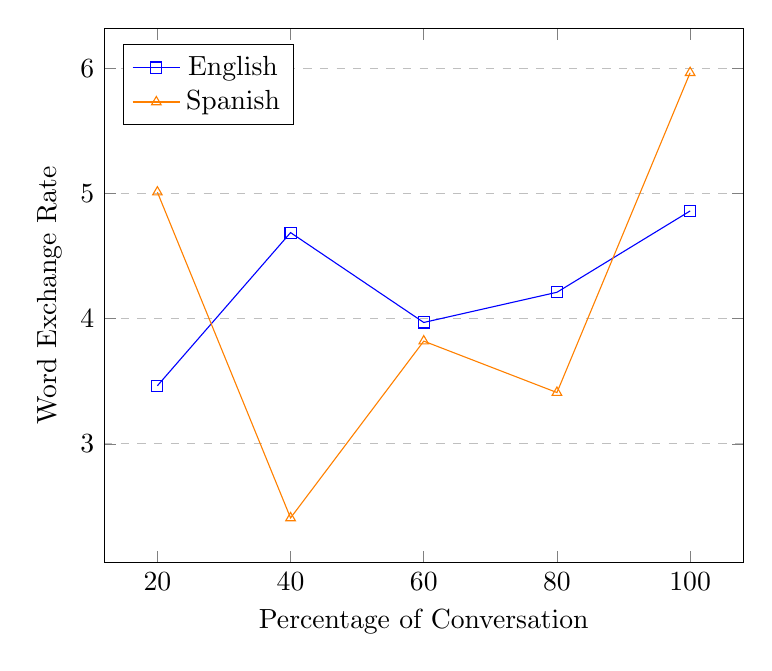
\begin{tikzpicture}
\begin{axis}[
    width=.8\columnwidth,
    xlabel={Percentage of Conversation},
    ylabel={Word Exchange Rate},
    xtick={20,40,60,80,100},
    ytick={2, 3, 4, 5, 6},
    legend pos=north west,
    ymajorgrids=true,
    grid style=dashed,
]

\addplot[
    color=blue,
    mark=square,
    ]
    coordinates {
    (20,3.464642667225855)
    (40,4.687988709000965)
    (60,3.9701977312366576)
    (80,4.2114241957197915)
    (100,4.860977398525937)
    };
    \addlegendentry{English}
    \addplot[
    color=orange,
    mark=triangle,
    ]
    coordinates {
    (20,5.011056181021869)
    (40,2.4085142391127423)
    (60,3.821182476393564)
    (80,3.410366654243342)
    (100,5.965185643313296)
    
    };
    \addlegendentry{Spanish}

\end{axis}
\end{tikzpicture}
\caption{Mean word exchange rates across Spanish and English conversations.} \label{fig:exchange-rate}
\end{figure}
%\vskip -0.5in

% \noindent
% \textbf{Linguistic synchrony.}  As a means to explore whether Spanish counselors adapt their language to synchronize with their patients, as done by their English-speaking counterparts, we measure the linguistic style matching (LSM) \cite{ireland2010language} in the conversations. LSM measures how much one speaker matches the other speaker's words while coordinating toward achieving a common goal (behavior change in this case). Previous work has found that linguistic coordination is a relevant determinant of psychotherapy treatment outcome~\cite{aafjes2020language}. We calculate LSM using the function categories from the LIWC lexicon. Results are shown in Figures \ref{fig:exchange-rate} and \ref{fig:lsm}.

% % We note that the LSM for both English and Spanish drops overall across the conversation, but for Spanish, the final 10\% of the sessions on average end with a bump in alignment, whereas English LSM steadily declines. Generally, the LSM for Spanish is higher than English. 

% %TODO revise
% From Figure \ref{fig:lsm}, we note that Spanish LSM scores exhibit a downward trend as the conversation progresses. Spanish conversations begin with higher LSM scores, indicating greater linguistic synchronization, but fluctuate significantly in the middle-to-late portions (30\%-80\%) before declining. English conversations also show some variability, with noticeable bumps in alignment around 40\% and 80\%. By the end of the conversation, LSM scores in both languages converge to similar levels.


% % LSM:
% \begin{figure}[!t]
% \centering
% \begin{tikzpicture}
% \begin{axis}[
%     width=\columnwidth,
%     xlabel={Percentage of Conversation},
%     ylabel={LSM Score},
%     % xmin=0, xmax=100,
%     % ymin=0.62, ymax=0.70,
%     xtick={20,40,60,80,100},
%     ytick={0.42,0.44,0.46,0.48,0.50,0.52,0.54,0.56,0.58},
%     legend pos=north east,
%     ymajorgrids=true,
%     grid style=dashed,
% ]

% \addplot[
%     color=blue,
%     mark=square,
%     ]
%     coordinates {
%     (0,0.5218041225968674)
%     (20,0.4602007355950078)
%     (40,0.4771863883255696)
%     (60,0.4651898578414786)
%     (80,0.4716878690621835)
%     };
%     \addlegendentry{English}

%     \addplot[
%     color=orange,
%     mark=triangle,
%     ]
%     coordinates {
%     (0,0.5613211876515827)
%     (20,0.48328694133005096)
%     (40,0.42605783465853797)
%     (60,0.4746430961897655)
%     (80,0.43519023887015623)
%     };
%     \addlegendentry{Spanish}

% \end{axis}
% \end{tikzpicture}
% \caption{LSM scores across Spanish and English conversations.} \label{fig:lsm}
% \end{figure}

% \begin{figure}[!t]
% \centering
% \begin{tikzpicture}
% \begin{axis}[
%     width=\columnwidth,
%     xlabel={Percentage of Conversation},
%     ylabel={LSM Score},
%     xmin=0, xmax=100,
%     ymin=0.62, ymax=0.78,
%     xtick={0,10,20,30,40,50,60,70,80,90,100},
%     ytick={0.62,0.64,0.66,0.68,0.70,0.72,0.74,0.76,0.78},
%     legend pos=north east,
%     ymajorgrids=true,
%     grid style=dashed,
% ]

% \addplot[
%     color=blue,
%     mark=square,
%     ]
%     coordinates {
%     (10,0.6683512766242292)
%     (20,0.6620906071020941)
%     (30,0.6356967993127416)
%     (40,0.6593838564410367)
%     (50,0.6473055064871894)
%     (60,0.6420047141356771)
%     (70,0.6444176877742241)
%     (80,0.6502999913193267)
%     (90,0.6373832889656631)
%     };
%     \addlegendentry{English}

%     \addplot[
%     color=orange,
%     mark=triangle,
%     ]
%     coordinates {
%     (10,0.7669285970879184)
%     (20,0.7469434695798091)
%     (30,0.7551817669014942)
%     (40,0.7293723051701744)
%     (50,0.72071575174295)
%     (60,0.7320142600828413)
%     (70,0.7279266330691515)
%     (80,0.7043829778247129)
%     (90,0.7179237728561156)
%     };
%     \addlegendentry{Spanish}

% \end{axis}
% \end{tikzpicture}
% \caption{LSM scores across Spanish and English conversations (using the first LIWC dataset).} \label{fig:lsm-old-spanish-data}
% \end{figure}

% \begin{figure}[!t]
%     \centering
% \includegraphics[width=\columnwidth]{figures/lsm.png} \caption{LSM across Spanish and English conversations.} \label{fig:lsm}
%  \end{figure}


 % English table:

% \begin{table}[t]
% \centering
% \small
% \resizebox{\columnwidth}{!}{%
% \begin{tabular}{l|cc|cc|cc} \hline
% {\multirow{2}{*}{Speaker}} &\multicolumn{2}{|c|}{Words}    &\multicolumn{2}{|c|}{Turns}   &\multicolumn{2}{|c}{Words/turn}\\ \cline{2-7}
%                     &Avg       &SD                 &Avg       &SD                    &Avg       &SD    \\ \hline

% Counselor    &  849.78   & 465.26   &  30.68   &  18.55   &  27.69   & 33.07 \\
% \hline
% Client    &  708.14  &  430.26  &  30.80   &  20.67   &  22.98   & 33.59 \\ 
% \hline 
% All     & 1557.92 & 782.79 & 61.49  & 38.94  & 25.33 & 33.42 \\ \hline
% \end{tabular}
% }
% \caption{Word-level and turn-level statistics for counselors and clients in the English counseling dataset. }
% \label{tab:word-turn-stats-en}
% %\vskip -0.2in
% \end{table}


% Spanish table:

% \begin{figure}[!t]
%     \centering
% \includegraphics[width=\columnwidth]{figures/session_by_length.png} \caption{Distribution of session lengths by number of turns for both Spanish and English datasets.} \label{fig:session-by-len}
%  \end{figure}% English table:





% \begin{figure}[!t]
%     \centering
% \includegraphics[width=\columnwidth]{figures/session_by_length.png} \caption{Distribution of session lengths by number of turns for both Spanish and English datasets.} \label{fig:session-by-len}
%  \end{figure}


%\subsection{Conversation-level Analyses}
%We also conduct conversation-level analysis, focusing on language usage and the sentiment and empathy expressed during the conversations. Again, we contrast our findings for Spanish MI with conversational trends seen in English MI.  

% \begin{table*}[]
% \centering
% \small
% %\resizebox{\textwidth}{!}{%
% \begin{tabular}{lll}
% \hline
% \multicolumn{3}{c}{\textbf{English}} \\ \hline
% {\ul Topic}            & {\ul Sample Tokens}                              & {\ul Distribution} \\ \hline
% Social Life            & friends, party, boss, kids, school, stress, risk & 15.89\%            \\
% Health Outlooks        & drinking, change, goal, life                     & 12.36\%            \\
% Medical Considerations & doctor, medication, smoking, family              & 34.10\%            \\
% Routines and Health    & day, time, week, breakfast, morning              & 8.77\%             \\
% Diabetes and Nutrition  & insulin, carbohydrates, diabetes, vegetables                   & 16.56\% \\
% Exercise               & exercise, basketball, weight                     & 8.77\%             \\
% Relationships          & future, arguments, relationship, mom             & 3.54\%             \\ \hline
% \multicolumn{3}{c}{\textbf{Spanish}}                                                           \\ \hline
% {\ul Topic}            & {\ul Sample Tokens}                              & {\ul Distribution} \\ \hline
% Wellness               & ejercicio, salud, doctor, cambio                 & 11.31\%            \\
% Time and Changes       & tiempo, cambio, vida, proceso, tratamiento       & 21.07\%            \\
% Cognitive Processes    & cuestion, riesgo, ansiedad, pensamiento          & 5.96\%             \\
% Relationships and Time  & padres, sentido, angustia, relacion, novio, semana, anos, vida & 25.66\% \\
% Diet and Nutrition      & dieta, diabetes, fruta, carbohidratos, comida                  & 13.69\% \\
% Alcohol                & alcohol, doctor, consumo, riesgo                 & 9.93\%             \\
% Stress on Relationships & consumo, hijos, proceso, amigos, trabajo, casa                 & 12.41\% \\ \hline
% \end{tabular}%
% %}
% \caption{Topic distributions across both languages. }
% \label{tab:topics}
% \end{table*}



%Seeking to further explore linguistic differences in counseling interactions in Spanish, we conduct word-based comparisons using the categories from the LIWC lexicon. 


\begin{table*}[t]
    \centering
    \small
\begin{tabular}{lcl|lcl}
\hline
% \small
\multicolumn{6}{c}{\textbf{Spanish}}\\ \hline	
 \multicolumn{3}{c}{Counselor} & \multicolumn{3}{c}{Client} \\ \hline
 You	&	4.89	&	tu, te, le, usted	&	I	&	4.57	&	yo, conmigo, mi, me	\\
Future	&	3.46	&	enfocaremos, hablaremos, podremos	&	Negate	&	2.29	&	ni, tampoco, nunca, no	\\
We	&	2.34	&	nos, nosotros, nuestra	&	Anger	&	2.06	&	problema, malo, molesta	\\
%Social	&	1.47	&	familiares, amigos, pelear	&	Home	&	1.81	&	familiares, casa,hogar	\\
Achieve	&	1.44	&	dejar, plan, mejorar, controlar	&	Family	&	1.63	&	familiar, padres, hijos	\\
%They	&	1.34	&	ellos,les, sus	&	Sad	&	1.54	&	triste, llorar, fracasar	\\
%See	&	1.27	&	vemos, observar, mirar, mira	&	Friend	&	1.49	&	amigo(a), pareja, novio(a)	\\
Insight	&	1.27	&	sientes, consideras	&	Negemo	&	1.49	&	enojado, ansiedad, decepcion	\\
%Preps	&	1.22	&	en, hasta, con, de	&	Adverb	&	1.48	&	ya, como, realmente	\\
Ipron	&	1.21	&	algunos, todos,estas, que	&	Conj	&	1.41	&	pues, y, cuando	\\
Inhib	&	1.16	&	dejar, evitar, control	&	Assent	&	1.41	&	verdad, acuerdo, bien	\\
%Relativ	&	1.14	&	parte, dentro, hagas	&	Excl	&	1.34	&	tampoco, sin, o	\\



\hline
\multicolumn{6}{c}{\textbf{English}}\\ \hline		
\multicolumn{3}{c}{Counselor} & \multicolumn{3}{c}{Client} \\ \hline	
You	&	2.04	&	yours, your, you	&	I	&	2.23	&	me, I, myself	\\
We	&	1.59	&	we, us, our	&	Home	&	2.08	&	family, house, room	\\
Cause	&	1.43	&	how, change, control	&	Friend	&	1.67	&	friend, college, partner	\\
%Social	&	1.42	&	family, talk, tell	&	Shehe	&	1.64	&	her, he, she, his	\\
Hear	&	1.36	&	sounds, said, hearing	&	Family	&	1.62	&	son, daugher, father, wife	\\
Achieve	&	1.25	&	control, work, able	&	Negate	&	1.46	&	won't, shoudn't, didn't	\\
Percept	&	1.19	&	looking, sound, feel, heard	&	Leisure	&	1.35	&	drinking, playing, exercising	\\
%Preps	&	1.16	&	during,thought, around	&	They	&	1.34	&	them, they, themselves	\\
%Relativ	&	1.10	&	moment, slowly,already 	&	Excl	&	1.25	&	or, if, not, really	\\
%Affect	&	1.10	&	success,problem, worried	&	Past	&	1.18	&	wanted, done, been	\\
Posemo	&	1.10	&	better, important, fun	&	Discrep	&	1.17	&	if, could, need	\\
%Anger	&	1.10	&	annoyed, angry, frustrated	&	Humans	&	1.16	&	people, kids, friends	\\


\hline\end{tabular}
 \caption{Results from LIWC word class analysis counselor and client interaction in Spanish and English.}
\label{tab:dominance1}

\end{table*}



\noindent \textbf{Language Usage. } We examine language differences using semantic classes from the Linguistic Inquiry and Word Count (LIWC) lexicon \cite{liwc} as a bridge between English and Spanish. The analysis using the Spanish and English LIWC and the word class scoring method of ~\cite{mihalcea2009linguistic} compares the major word categories used by counselors and clients during the conversations. Table~\ref{tab:dominance1} shows the main word classes, with examples,  associated to counselors and clients in both languages. 

Counselors in both languages generally use words related to \textit{you}, \textit{we}, \textit{social}, and \textit{achieve}, which are relevant for MI. However, Spanish MI counselors focus more on \textit{Future} and \textit{Inhib} (inhibition) words. English MI counseling features more \textit{hear} and \textit{percept} (perception) words. These differences could also be related to culture, as in many Spanish-speaking countries healthcare providers take a more authoritative or directive approach to their patients ~\cite{coulter2003european,GimnezMoreno2022TheEO}. In addition,  clients also exhibit similar language use, such as \textit{I}, \textit{Home}, \textit{Family}, \textit{Negate}, with notable differences: Spanish clients use \textit{assent} words, while English clients use \textit{discrep} (discrepancy) words, suggesting greater compliance by Spanish clients.
%The LIWC dictionaries for English and Spanish share the same 64 categories. The English dictionary comprises 4,071 words, while the Spanish dictionary includes 12,421.








 
% Our analysis begins by counting the frequency of each LIWC category within the English and Spanish datasets. We then identify the top 10 most common categories for each language. To ensure comparability across languages, we normalize the frequency of each category by the total word count in the respective language dataset. The distribution of these LIWC categories is presented in Fig. \ref{fig:liwc-top-10-all}, where we observe that words related to cognitive processes are highly common in both languages, second only to function words. In addition, we find that Spanish conversations exhibit an overall higher frequency of pronoun usage compared to English, as indicated by taller bars for the ``pronoun'', ``ppron'', and ``ipron'' categories. To gain some general cross-language comparisons, we also map each category to four higher dimensions according to \cite{liwc}: (1) Linguistic Processes (LIN),
% (2) Psychological Processes (PSY), (3) Personal Concerns (PER), and (4) Spoken categories (SPOKEN). Our findings in Figures \ref{fig:liwc-dim-all}, \ref{fig:liwc-dim-counselor}, and \ref{fig:liwc-dim-patient} show that the LIN and PSY dimensions are the most dominant across both languages and speaker roles, with Spanish dialogues showing a slightly higher frequency in the PSY dimension. We find interesting patterns on pronoun usage, so we wonder what are the most common pronouns.
% This suggests a nuanced difference in the expression of psychological content between English and Spanish, potentially reflecting cultural or linguistic influences in counseling practices.
% Following this mapping, Fig. \ref{fig:dim-all} depicts the distribution of dimensions in English and Spanish conversations.

% The LIWC analysis reveals several interesting patterns across languages and speaker roles. When comparing English and Spanish conversations (Fig. \ref{fig:dim-all}), English has over 50\% of words falling under the ``language'' dimension. This is much higher than Spanish, and is likely due to the frequent usage of function words in English that are missing in the Spanish LIWC dictionary (Fig. \ref{fig:liwc-top-10-all}). In addition, both languages show a focus on the present moments and relatively low mentions of current concerns (Figs. \ref{fig:dim-counselor}, \ref{fig:dim-patient}). 

% In terms of speaker roles, counselors generally use second-person pronouns such as ``you'' more frequently than patients during therapy sessions (Table \ref{tab:patient-pronoun}, \ref{tab:couneslor-pronoun}). In contrast, patients, particularly in Spanish, use first-person singular pronouns like ``I'' more often, indicating their tendency for self-focused conversations (Figure \ref{fig:cat-sp}). This finding aligns with \citet{pennebaker_secret_2013} that individuals experiencing depression tend to use first-person pronouns more frequently; this also indicates higher-quality counseling \cite{perez-rosas-etal-2017-understanding}. 
% Further analyses in LIWC are presented in section \ref{subsec:more-liwc}. 

% \begin{figure}[t]
%     \centering
% \includegraphics[width=0.8\columnwidth]{figures/counselor_sentiment_barplot.png} \caption{Distribution of counselor sentiment over the conversation duration} 
% \label{fig:counselor-sentiment-barplot}
%  \end{figure}
%  %\vskip -0.5in


\begin{figure}[t]
    \centering
\includegraphics[width=.9\columnwidth]{figures/counselor_sentiment_boxplot_full_scale.png} \caption{Counselor sentiment across languages} 
\label{fig:counselor-sentiment-boxplot}
 \end{figure}

 
\noindent \textbf{Sentiment Trends.}
\label{sec:sentiment} The sentiment exhibited by counselors can reflect their empathy and responsiveness, which are important factors for positive treatment outcome \cite{eberhardt2024decoding,perez-rosas-etal-2019-makes}. %Similarly, patients' sentiments can reveal their emotional states.
%We analyze the sentiment expressed by counselors across the two languages. %, examining both language (English and Spanish) and speaker role (counselor vs. patient). 
We use the multilingual PySentimiento library \cite{perez2021pysentimiento} to obtain positive, neutral, and negative sentiment scores on conversational turns. To further evaluate the performance of the sentiment classifier in Spanish data, we randomly sample 10\% (300) of 3,018 Spanish utterances and independently annotate them for sentiment using the same categories. The annotation is conducted by two native Spanish speakers, achieving a Cohen kappa of 0.45 and a raw agreement of 0.64, indicating moderate agreement. A third native speaker conducted further attribution on 107 utterances with disagreement. Among the 300 utterances, the classifier correctly classifies 192, yielding an accuracy of 0.64. Notably, most misclassifications (69 out of 109) occur when the classifier predicts neutral sentiment. Given reasonable accuracy scores, we use classifier predictions to conduct sentiment comparisons across both languages. Figure \ref{fig:counselor-sentiment-boxplot} illustrates the distribution of counselor sentiment, showing that neutral sentiment is the most prevalent in both languages, while positive and negative sentiments occur more frequently in Spanish conversations. 







% To examine how positive sentiment evolves during counselor-patient interactions, we divided each session into five stages containing a nearly equal number of turns, following the methodology of \cite{perez-rosas-etal-2019-makes}. The average turn length for each stage is detailed in Appendix \ref{subsec:sentiment}, Fig \ref{fig:turn-len-eng} and \ref{fig:turn-len-sp}. 

% We hypothesize that sessions would generally exhibit a trend toward increasing positive sentiment. To test our hypothesis, we divide the turns in each session into five splits and calculated the frequency of positive sentiment at each stage. 

% We also examined the trend of sentiment expressed by counselors throughout the conversation. To do this, we divide the counselor dialogues in each session into five splits and calculate the distribution of positive sentiment
%  at each stage. %As illustrated in Figure \ref{fig:pos-split-all}, both the English and Spanish conversations show a U-shaped pattern,  suggesting that counselors and patients in both languages tend to begin and end conversations with more positive remarks and that the middle of the conversation might address issues with less positive sentiment. 
% %Furthermore, 


% In Figure \ref{fig:counselor-sentiment-boxplot}, we plot the sentiment counselors express across languages. We observe that English counselors make positive remarks more often than their Spanish counterparts.%, a trend mirrored among patients as shown in Figure \ref{fig:patient-sentiment-boxplot}. 
% In addition, Figure \ref{fig:counselor-sentiment-barplot} shows a noticeable increase in positive sentiment in the latter half of English conversation. However, a U-shaped curve is observed in both languages. %Figures \ref{fig:sentiment-speaker-en} and \ref{fig:sentiment-speaker-sp} indicate that counselors in both languages generally use more positive language than patients during the early stages of the conversation, but this difference diminishes towards the end. %Regarding neutral and negative sentiments, the plots in Appendix \ref{sec:sentiment-more} demonstrate an opposite trend to positive sentiment, with both neutral and negative sentiments increasing in the first half and decreasing in the second half. Notably, patients in both languages, especially Spanish, tend to use more neutral language than counselors, while both speaker roles employ comparable levels of negative remarks (Fig \ref{fig:neutral-en}, \ref{fig:neutral-sp}, \ref{fig:negative-en}, and \ref{fig:negative-sp}).      

 

% The sentiment scores for positive, neutral, and negative sentiments for counselors and patients are shown in Appendix \ref{subsec:three-sentiments-en}, Fig \ref{fig:three-sent-counselor} and \ref{fig:three-sent-patient}.   



% \begin{figure}[t]
%     \centering
% \includegraphics[width=\columnwidth]{figures/pos_sent_couns.png} \caption{Distribution of \textbf{positive} sentiment of the counselor in each 20\% conversation
% splits.} \label{fig:pos-split-couns}
%  \end{figure}

%  \begin{figure}[t]
%     \centering
% \includegraphics[width=\columnwidth]{figures/pos_sent_patient.png} \caption{Distribution of \textbf{positive} sentiment of the patient in each 20\% conversation
% splits.} \label{fig:pos-split-pat}
%  \end{figure} 

 
% \begin{figure}[t]
%     \centering
% \includegraphics[width=\columnwidth]{figures/pos_sent_couns.png} \caption{Distribution of \textbf{positive} sentiment of the counselor in each 20\% conversation
% splits.} \label{fig:pos-split-couns}
%  \end{figure}

%  \begin{figure}[t]
%     \centering
% \includegraphics[width=\columnwidth]{figures/pos_sent_patient.png} \caption{Distribution of \textbf{positive} sentiment of the patient in each 20\% conversation
% splits.} \label{fig:pos-split-pat}
%  \end{figure}


%compare broadly to empathy shown by counselors speaking English 

% \subsection{Empathy}

% Counselor empathy is also relevant to counseling quality \cite{redfern1993empathy}. We explore differences in empathetic behaviors between Spanish and English MI counselors. Given that counseling datasets examined in this paper do not include empathy annotations, we obtained conversation-level synthetic empathy assessments by training a multilingual empathy classifier using MLBERT~\cite{DBLP:journals/corr/abs-1810-04805}. 
% We fine-tune the empathy model using the English counseling dataset contributed by \cite{perez-rosas-etal-2017-understanding}, which contains empathy assessments on actual MI conversations on a Likert scale of 1 (least empathetic) to 5 (most empathetic). We apply the empathy classifier on the aggregate counselor utterances for each transcript in both datasets, and results are visualized in \ref{fig:empathy-table}.

% Overall, counselors in both languages exhibit moderate levels of empathy. However, there is a little more variety among Spanish counselors, with several conversations showing lower empathy scores (score of 2).  

% \begin{figure}[h!]
%     \centering   \includegraphics[width=\columnwidth]{figures/empathy_counselor_only.png}
%     \caption{Empathy scores on the Spanish and English datasets.}
%     \label{fig:empathy-table}
% \end{figure}

%We note that this portion of our study is intended to broadly understand differences in empathy expressed in our English and Spanish datasets rather than to come to conclusive judgments, as the empathy annotations are collected from real MI sessions with only English-speaking participants so they may not directly translate to our datasets of interest, both sourced from the internet. 


\begin{table*}[t!]
\centering
\small
%\resizebox{\textwidth}{!}{%
\begin{tabular}{lll|ll|ll|ll}
\multicolumn{5}{c}{{ \textbf{Monolingual Models}}} & \multicolumn{4}{c}{{ \textbf{Multilingual Models}}} \\ \hline
              & \multicolumn{2}{c}{en-BERT} &        \multicolumn{2}{c}{sp-BETO}       & \multicolumn{2}{c}{en-MLBERT} &        \multicolumn{2}{c}{sp-MLBERT}        \\ \cline{2-9}
              
              & 2-way   & 3-way & 2-way   &   3-way & 2-way     & 3-way & 2-way     & 3-way \\ \cline{1-9} 
Accuracy      & .83   & .88 & .92        & \multicolumn{1}{l|}{.92} & .77     & .89 & .84    & .89 \\ \hline
F1            & .82   & .88 & .92        & \multicolumn{1}{l|}{.92} & .76     & .88 & .84     & .88 \\ \hline
F1-Other       & -       & .95   & -            & \multicolumn{1}{l|}{.90}   & -         & .96   & -         & .95   \\ \hline
F1-Question   & .88     & .65   & .95 & \multicolumn{1}{l|}{.89}   & .84       & .63   & .90       & .54   \\ \hline
F1-Reflection & .64     & .46   & .82 & \multicolumn{1}{l|}{.66}   & .57       & .29   & .68       & .22   \\ \hline
\end{tabular}%
%}
    \caption{ Classification results using monolingual models (sp-BETO, en-BERT) and multilingual models (sp-MLBERT, en-MLBERT) for 2-way (reflection vs question) and 3-way (Question vs Reflection vs Other) classification. Notations in the form \{language-\textsc{model}\} indicate in which language the model is fine-tuned on.}
    \label{tab:3way}
\end{table*}
%In addition to topic modeling, we gain a more granular

\section{Predicting Counselor Behaviors}

In addition to linguistic analyzes, we perform classification experiments in Spanish and English conversations to classify counselor behavior using MIDAS and its English counterpart, described in Section 4. Similarly to the label classification experiments in \cite{hebrew-counseling}, we define two tasks: binary classification to differentiate reflections from questions, and three-way classification to identify questions, reflections, or neither. 
We experiment with two settings: we train and test the classifiers using the same language for both the training and the test data; and we use multilingual language models to enable training on one language and evaluation on the other.
%Our experiments are structured as a classification task on annotated MITI labels––our models are trained and evaluated on how well they are able to predict if a provided utterance is a question, reflection, or neither. 
% We evaluate both monolingual and cross-lingual experimental settings. We use the Spanish and English datasets described in Section \ref{section-data-collection} during our experiments and English translations of the Spanish dataset, obtained using Google Cloud Translate API. \footnote{\href{https://console.cloud.google.com/marketplace/product/google/translate.googleapis.com}{Google Cloud Translate API}} 
% The classification experiments are evaluated using monolingual and multilingual models. %Both types of models are used to evaluate monolingual experiments, and only the multilingual model can enable multilingual experiments.  
% \noindent
% \textbf{Monolingual Experiments. } 
% \noindent
% \textbf{Multilingual Experiments.} 
%During our experiments, we use the Spanish and English datasets described in Section \ref{section-data-collection}. %For comparison, we provide results of fine-tuning monolingual models; i.e. the source and target languages are the same.
%The experiments include the following set-ups:
% the monolingual model is trained and evaluated on the same language,
% the monolingual model is trained on original data of one language and evaluated on machine-translated data of the other language, 
% the multilingual model is trained and evaluated on the same language, or
% the multilingual model is trained on one language and evaluated on the other language. 



For our experiments, we use a 85\%--15\% training--test split. 
%We use a 15\% split for hyperparameter-tuning. 
For the monolingual experiments, as our main models we use BERT  \cite{devlin2018bert} and BETO \cite{cañete2023spanish}, a BERT architecture trained on Spanish text.
For the multilingual experiments, we use a BERT architecture trained for multiple languages, including English and Spanish BERT \cite{DBLP:journals/corr/abs-1810-04805}, denoted as ML-BERT. We attach classification heads to the base models and fine-tune each model for five epochs each. Results for the classification experiments
%when training and evaluating in the same language and different language 
are shown in Table \ref{tab:3way}. 




%We attach classification heads to the base models and fine-tune each model for five epochs each.

% Please add the following required packages to your document preamble:
% \usepackage{graphicx}
% \usepackage[normalem]{ulem}
% \useunder{\uline}{\ul}{}

% % Please add the following required packages to your document preamble:
% % \usepackage{graphicx}
% \begin{table}[]
% \centering
% \small
% % \resizebox{\columnwidth}{!}{%
% \begin{tabular}{lllll}
%          & \multicolumn{2}{l}{en-sp MLBERT} & \multicolumn{2}{l}{sp-en MLBERT} \\ \cline{2-5} 
%          & 2-way           & 3-way          & 2-way           & 3-way          \\ \cline{2-5} 
% Accuracy &  .75            & .71            &     .74          &  .82              \\ \hline
% F1       &  .76              & .63            &  .72               &  .75              \\ \hline
% F1-Other &       -          & .84            &      -           &  .09            \\ \hline
% F1-Quest &   .82            & .05            &   .83              &  .03            \\ \hline
% F1-Ref   &    .63             & .03            &    .42            &   .01           \\ \hline
% \end{tabular}%
% %}
% \caption{Results from fine-tuning MLBERT on a source language and evaluating on a target language (e.g., en-sp denotes English as the source and Spanish as the target). }
% \label{tab:mlbert-different-source-target-results}
% \end{table}

% \begin{table}[]
%     \centering
%     \small
%     \begin{tabular}{l|ccc}
%     \hline
%    Model & Acc. &  F1-Quest &  F-Ref \\ \hline
%    sp-BETO & \textbf{.92} & \textbf{.95} & \textbf{.82} \\
%    en-BERT      &  .83 & .88 & .64 \\
%    sp-MLBERT & .84 & .90 & .68 \\  \hline
%     \end{tabular}
%     \caption{  Monolingual (sp-BETO) and cross-lingual classification (en-BERT, en-MLBERT) results for binary (Quest vs Ref) classification}
%     \label{tab:2way}
% \end{table}


% \begin{table}[]
%     \centering
%     \small
%     \begin{tabular}{l|cccc}
%     \hline
%    Model & Acc. &  F1-Quest &  F-Ref  & F-Other\\ \hline
%      sp-BETO & \textbf{.90} & \textbf{.89} & \textbf{.66}  & \\
%    en-BERT      &  .87 & .56 & .45 &  \\
%    sp-MLBERT & .88 & .54 & .22 \\  \hline
%    \end{tabular}
%     \caption{ Monolingual (sp-BETO) and cross-lingual classification (en-BERT, en-MLBERT) results for 3-way (Quest vs Ref vs Other) classification}
%     \label{tab:3way}
% \end{table}

% \begin{table*}[h]
% \centering
% \resizebox{\textwidth}{!}{%
% \begin{tabular}{lllllllll}
% \multicolumn{5}{l}{{\ul \textbf{Monolingual Models}}} & \multicolumn{4}{l}{{\ul \textbf{Multilingual Models}}} \\
%               & en-BERT &       & sp-BETO      &       & en-MLBERT &       & sp-MLBERT &       \\ \cline{2-9} 
%               & 2-way   & 3-way & 2-way        & 3-way & 2-way     & 3-way & 2-way     & 3-way \\ \cline{2-9} 
% Accuracy      & .8252   & .8723 & .9207        & .9017 & .7669     & .8891 & .8417     & .8874 \\ \hline
% F1            & .8228   & .8670 & .9222        & .9008 & .7643     & .8815 & .8433     & .8834 \\ \hline
% F1-question   & .88     & .56   & \textbf{.95} & .89   & .84       & .63   & .90       & .54   \\ \hline
% F1-reflection & .64     & .45   & \textbf{.82} & .66   & .57       & .29   & .68       & .22   \\ \hline
% \end{tabular}%
% }
% \caption{Baseline results for classification using monolingual BERT models and multilingual BERT model; F1 is the weighted average across labels. Best results per class for each of the 2-way and 3-way experiments are bolded. }
% \label{tab:bert-results}
% \end{table*}


% \begin{table*}[h]
% \centering
% \scriptsize
% \resizebox{\textwidth}{!}{%
% \begin{tabular}{lllll}
%          & en-BERT & sp-BETO & en-to-sp-BETO & sp-to-en-BERT \\ \cline{2-5} 
% Accuracy & \textbf{0.8174} & 0.8057 & 0.7927 & 0.7395 \\ \hline
% F1       & 0.7757 & \textbf{0.7975} & 0.7741 & 0.6737  \\ \hline
% \end{tabular}%
% }
% \caption{Results of p-tuning on BERT and BETO.}
% \label{tab:MIbert-ptuning}
% \end{table*}

% \begin{table*}[H]
% \centering
% \resizebox{\textwidth}{!}{%
% \begin{tabular}{lllll}
%         & en-MLBERT & sp-MLBERT & en-to-sp-MLBERT & sp-to-en-MLBERT \\ \cline{2-5} 
% Accuracy & \textbf{0.8041} & 0.7704 & 0.7946 & 0.6622 \\ \hline
% F1       & 0.7440 & 0.7267 & \textbf{0.7642 }& 0.5532  \\ \hline
% \end{tabular}%
% }
% \caption{Results of p-tuning on MLBERT.}
% \label{tab:mlbert-ptuning}
% \end{table*}


% \begin{table*}[]
% \centering
% \resizebox{\textwidth}{!}{%
% \begin{tabular}{lllllllll}
% \multicolumn{9}{l}{{\ul \textbf{Monolingual Models}}} \\ \hline
%  &
%   \multicolumn{2}{l}{en-BERT} &
%   \multicolumn{2}{l}{sp-BETO} &
%   \multicolumn{2}{l}{en-to-sp-BETO} &
%   \multicolumn{2}{l}{sp-to-en-BERT} \\ \cline{2-9} 
%  &
%   Question &
%   \multicolumn{1}{l|}{Reflection} &
%   Question &
%   \multicolumn{1}{l|}{Reflection} &
%   Question &
%   \multicolumn{1}{l|}{Reflection} &
%   Question &
%   Reflection \\ \cline{2-9} 
% Label-Specific F1 &
%   .87 &
%   \multicolumn{1}{l|}{.72} &
%   .81 &
%   \multicolumn{1}{l|}{.72} &
%   .84 &
%   \multicolumn{1}{l|}{.60} &
%   .89 &
%   .71 \\ \hline
% {\ul \textbf{Multilingual Models}} &
%    &
%    &
%    &
%    &
%    &
%    &
%    &
%    \\ \cline{1-1}
%  &
%   \multicolumn{2}{l}{en-MLBERT} &
%   \multicolumn{2}{l}{sp-MLBERT} &
%   \multicolumn{2}{l}{en-to-sp-MLBERT} &
%   \multicolumn{2}{l}{sp-to-en-MLBERT} \\ \cline{2-9} 
%  &
%   Question &
%   \multicolumn{1}{l|}{Reflection} &
%   Question &
%   \multicolumn{1}{l|}{Reflection} &
%   Question &
%   \multicolumn{1}{l|}{Reflection} &
%   Question &
%   Reflection \\ \cline{2-9} 
% Label-Specific F1 & .81 & \multicolumn{1}{l|}{.57} & .92 & \multicolumn{1}{l|}{.77} & .82 & \multicolumn{1}{l|}{.51} & \multicolumn{1}{l|}{.79} & \multicolumn{1}{l|}{.52} \\ \hline
% \end{tabular}%
% }
% \caption{Label-specific F1 scores for 2-way classification using baseline fine-tuned models. }
% \label{tab:bert-2way-f1s}
% \end{table*}

% \begin{table}[h!]
% \centering
% \resizebox{\columnwidth}{!}{%
% \begin{tabular}{lll}
%          & en-on-sp-MLBERT & sp-on-en-MLBERT \\ \cline{2-3} 
% Accuracy & 0.6423   & \textbf{0.7927}\\ \hline
% F1       & 0.5102   & \textbf{0.7334} \\ \hline
% \end{tabular}%
% }
% \caption{Continuation of Table \ref{tab:mlbert-ptuning} on ML-BERT with no machine translated training or evaluation data.}
% \label{tab:mlbert-ptuning-continued}
% \end{table}


% \begin{table*}[h]
% \centering
% \resizebox{\textwidth}{!}{%
% \begin{tabular}{lllllllll}
% \multicolumn{9}{l}{{%\ul 
% \textbf{Monolingual Models}}}                                                          \\ \hline
%          & \multicolumn{2}{l}{en-BERT}   & \multicolumn{2}{l}{sp-BETO}          & \multicolumn{2}{l}{en-to-sp-BETO}   & \multicolumn{2}{l}{sp-to-en-BERT}   \\ \cline{2-9} 
%          & 2-way   & 4-way    & 2-way            & 4-way            & 2-way   & 4-way    & 2-way     & 4-way   \\ \cline{2-9} 
% Accuracy & 0.712       & \textbf{0.804}      & 0.855 & 0.805 & ?          & 0.792         &   ?        & 0.739          \\ \hline
% F1       & 0.592 & 0.744 & 0.850 & 0.726 & ? & \textbf{0.764} & ? & 0.553  \\ \hline
% \multicolumn{9}{l}{{%\ul 
% \textbf{Multilingual Models}}}                                                         \\ \hline
%          & \multicolumn{2}{l}{en-MLBERT} & \multicolumn{2}{l}{sp-MLBERT}        & \multicolumn{2}{l}{en-to-sp-MLBERT} & \multicolumn{2}{l}{sp-to-en-MLBERT} \\ \cline{2-9} 
%          & 2-way   & 4-way    & 2-way            & 4-way            & 2-way   & 4-way    & 2-way     & 4-way   \\ \cline{2-9} 
% Accuracy & 0.712  & \textbf{0.804}    & 0.761  & 0.770  & ?  & 0.794   & ?    & 0.662  \\ \cline{2-9} 
% F1       & 0.592  & 0.744   & 0.701  & 0.726  & ?  & \textbf{0.764}   & ?   & 0.553 \\ \hline
% \end{tabular}%
% }
% \caption{P-tuning results for classification using monolingual BERT models and multilingual BERT model; F1 is the weighted average across labels.}
% \label{tab:ptuning-bert-results}
% \end{table*}


% \begin{table}[h]
% \centering
% \resizebox{\columnwidth}{!}{%
% \begin{tabular}{lllll}
%          & \multicolumn{2}{l}{en-on-sp-MLBERT}    & \multicolumn{2}{l}{sp-on-en-MLBERT} \\ \cline{2-5} 
%          & 2-way   & \multicolumn{1}{l|}{4-way}   & 2-way             & 4-way           \\ \cline{2-5} 
% Accuracy & ? & \multicolumn{1}{l|}{0.642} & ?           & \textbf{0.7927}          \\ \hline
% F1       & ? & \multicolumn{1}{l|}{0.510} & ?          & 0.733         \\ \hline
% \end{tabular}%
% }
% \caption{Continuation of Table \ref{tab:ptuning-bert-results} on ML-BERT with no machine-translated training or evaluation data.}
% \label{tab:ptuning-mlbert-results}
% \end{table}

%The utterances and their corresponding labels are determined by the annotated start and end positions; non-annotated text is classified as "none."
% Training on original English and testing on machine-translated Spanish-to-English is denoted as sp-to-en, and training on Spanish and testing on machine-translated English-to-Spanish is denoted as en-to-sp. 
%For multilingual BERT (ML-BERT), we additionally fine-tune on the original English data and evaluate on the original Spanish data, and vice versa––these are denoted as en-on-sp and sp-on-en, respectively. 

%We evaluate these set-ups for both binary classification for the two primary labels (questions and reflections; denoted as 2-way), as well as 3-way classification for the full set of possible labels (questions, reflections, none; denoted as 3-way).
% Results for the experiments with the BERT models on 2-way (question, reflection) and 4-way (question, reflection, combination, none) classification are in Table \ref{tab:bert-results}. Additionally, we provide individual F1 scores for the ``question'' and ``reflection'' labels in Table \ref{tab:bert-2way-f1s}. 

% \subsection{P-tuning}

% In addition to the baseline experiments in which we have a traditional fine-tuning set-up, we experiment with p-tuning \cite{p-tuning}. 
% When the labeled training data is insufficient––as is often the case for low-resource languages––prompt-tuning has been demonstrated as effective to induce knowledge from pre-trained language models \cite{uniprompt, brown_language_2020, gao-etal-2021-making, le-scao-rush-2021-many, zhao-schutze-2021-discrete}. 

%We use a 70\% 30\% training test split for p-tuning experiments. After experimenting with a few hyperparameters, we set the number of virtual tokens to 15 (num{$_$}virtual{$_$}tokens in PromptEncoderConfig) and encoder hidden size to 128 (encoder{$_$}hidden{$_$}size in PromptEncoderConfig). Same as baseline experiment, we finetune for 5 epochs before evaluation. In addition to these parameters, we investigate the impact of prompt length on model performance by experimenting with p-tuning using different numbers of virtual tokens (10, 20, 30, 40, and 50) in 4-way classification. Results for p-tuning experiments are available in Tables  \ref{tab:MIbert-ptuning}, \ref{tab:mlbert-ptuning},  and \ref{tab:mlbert-ptuning-continued}, 
 
% P-tuning  adds prompt embeddings to the input that are optimized by a prompt encoder during fine-tuning; rather than fine-tuning the entire model, only these added weights are updated during training. It has been shown to improve efficiency and even model performance in certain supervised settings. To better compare p-tuning and fine-tuning, we train the models for 5 epochs and use the same training-test split ratio as baseline experiments. More training details can be found in Appendix section \ref{subsec: p-tuning details}. To evaluate the relationship between prompt length and model performance, we experiment with 5 different number of virtual tokens in each p-tuning experiment: 10, 20, 30, 40, 50. Full results are plotted in section \ref{TODO}  
 
% \subsection{Results} \label{section-results}

%, \ref{tab:mlbert-different-source-target-results}. %The former includes results on training and evaluating in the same language, while the latter includes results on training and evaluating in different languages. 
In general, we observe that questions are easier to predict than reflections. This aligns with previous work done on English, where reflections were also more challenging to classify, and with work conducted on Hebrew \cite{hebrew-counseling} in which questions are easier to classify than other codes. 
%In general, when considering all models and experiments, the classification of the "Other" label performs better than the classification of the two MI labels. Additionally, the classification of the "question" label performs better than the classification of the "reflection" label. 
%These findings are consistent with the distribution of the labels across both languages and are further supported by the fact that specific question words can often be used to distinguish questions in text, which the models likely learn. 
An important take-away from our experiments is that performing training and evaluation  in the same language outperforms multilingual settings.%, agreeing with similar experiments for emotion classification in Polish \cite{polish-mh-dialogues}.
% We note that the 3-way classification results––\ref{tab:mlbert-different-source-target-results}––are less impressive than those of 2-way classification. It is possible that the models become over-reliant on predicting the ``none" label, due to its higher frequency in the dataset. 
%An important takeaway from our experiments is that best results are obtained when training and evaluating on the same language using a base model pre-trained in that language.  

 

%For the experiments conducted using machine-translated data, the best performance is exhibited with BETO trained on original Spanish data.
%evaluated on the English-to-Spanish translations data. 
%Strictly within languages, the fine-tuned monolingual models outperform their fine-tuned multilingual model counterparts. 

%We note that for both languages, the relative best performances are consistently made up solely of that language; i.e. regardless of model, English tags are best predicted using original English data, and Spanish tags are best predicted using original Spanish data. Machine-translated data used for training consistently worsens predictive performance. However, the machine-translated training procedure performs better for all models when compared to training ML-BERT on one language and evaluating on the other. 

%Based on 2-way classification results, we find that the ``question'' label is easier to predict compared to ``reflection'', regardless of language. This is likely attributed to the models learning the common structure of questions, as well as question words (e.g. ``why'', ``como''). 

% In summary, we find that training and evaluating on a single language is optimal for both Spanish and English, followed by training on machine-translations of the target language, followed by training a multilingual language model on one language and evaluating on the other.

% \subsection{P-tuning Results}

% P-tuning overall yields comparable and even better results than full fine-tuning in the majority of experiments. In cross-lingual transfer tasks, such as training on original Spanish and testing on original English text, p-tuning outperforms fine-tuning by over 10\%.     

% In addition, we find that the performance of p-tuning is impacted by prompt length. Specifically, either a long (more than 50 virtual tokens) and short (fewer than 20 virtual tokens) prompt is detrimental to model performance. The best prompt usually has 20 or 30 tokens. The full results are presented in section \ref{sec:prompt-length}.

\section{Conclusion}

In this work, 
we introduced MIDAS, a Motivational Interviewing Dataset in Spanish, the first Spanish MI dataset. We conducted comparative analyzes of the language used by counselors in Spanish and English counseling interactions and found differences in linguistic styles and conversation dynamics.  
Future work includes a more extensive analysis of the differences between English and Spanish counseling, including conversational dynamics such as verbal mirroring and power dynamics, as well as conversational strategies such as empathy or partnership. We also envision MIDAS as a valuable resource in building NLP applications to support counseling evaluation and training for Spanish speakers. 


% For example, MIDAS could be used to conduct more in-depth comparisons between MI in Spanish and English, such as studying the rates of reflection or question usage in successful and less successful conversations. 
% Toward \textbf{applications}, we envision using MIDAS on its own or to augment external datasets. For example, 
% MIDAS can be used to learn classifiers that can automatically annotate MI sessions with Spanish speakers, which can in turn be used for large-scale analysis or for training larger models. Additionally, since MIDAS has expert-annotated labels, models for cross-lingual label projection can be developed between Spanish and English, as well as Spanish and other annotated MI datasets.

% todo add a couple specific examples



The MIDAS dataset is publicly available under \url{https://github.com/MichiganNLP/MIDAS}. 



%todo future work
% -- want to contextualize; how SPECIFICALLY can MIDAS be used for downstream applications





\section{Limitations} % nec for NAACL

A limitation of this work is that the collected transcripts are sourced from online videos created for educational purposes and may be scripted to some extent. However, it is important to mention that in real counseling this is a common practice, as counseling training often makes use of actors who perform different learning scenarios. Although client behavior may be more unpredictable in real counseling, we believe that this dataset can provide important information for the study of the behavioral and cultural differences of Spanish counseling.

%rather for the development of cross-lingual projection methods and further comparison between English and Spanish MI.

% More limitations: 
% 1. We didn't try more parameter-efficient tuning techniques, since it's not a focus of this paper. For example, prefix tuning and LoRa aren't tested. Future researchers may do a more comprehensive analysis on different PEFT.  
% 2. We didn't fine-tune the pretrained model on sentiment

\section{Acknowledgments}
We are grateful to Marlene Reyes, Hector Pizarro, and Ana Ronquillo for assisting us with the data collection and the counseling annotations. We also thank the anonymous reviewers for their constructive feedback and the members of the Language and Information Technologies lab at the University of Michigan for the insightful discussions during the early stages of the project. This project was partially funded by a National Science Foundation award (\#2306372). Any opinions, findings, conclusions, or recommendations expressed in this material are those of the authors and do not necessarily reflect the views of the National Science Foundation.

\bibliography{anthology,custom}

% \appendix

% \section{Topic Distribution}

% \paragraph{Conversational Topics. }
% To broadly understand the types of issues discussed across conversations, we use Latent Dirichlet Allocation (LDA) topic modeling\footnote{https://radimrehurek.com/gensim/models/ldamodel.html} across English and Spanish nouns and verbs. We allocate seven topics for each language. Based on the resulting groups of words, we manually summarize the topics covered in each language and compute that topic's distribution across transcripts. The results for the topic extraction, including a few significant description tokens associated with each topic, are shown in Table~\ref{tab:topics}.

% \textit{Spanish}: 
% (1) alcohol consumption [alcohol, salud, dejar], 28.06\%;
% (2) relationships [familia, relación, casa], 10.86\%;
% (3) smoking [fumar, doctor, dejar], 23.94\%;
% (4) food and diet [consumo, proceso, azúcar], 6.97\%;
% (5) general drug use [fumar, beber, doctor], 13.51\%;
% (6) diabetes [azúcar, diabetes, glucosa, ejercicio], 16.64\%.

% \textit{English:}
% (1) blood pressure [blood, pressure, exercise, medication], 9.41\%;
% (2) alcohol consumption [drink, alcohol, quit], 9.47\%;
% (3) food and diet [eat, diet, breakfast, sugar, teeth], 42.01\%;
% (4) work [work, boss, week], 1.15\%;
% (5) cleanliness [asthma, dog, house, dust, clean], 28.14\%;
% (6) smoking [nicotine, quit, smoking], 9.78\%.

% We note that there isn't a significant difference in the types of topics discussed, but there are some slight differences in distribution. Spanish-speaking patients are more likely to discuss alcohol consumption and smoking, whereas English-speaking patients are more likely to discuss food and diet. 
% This can be attributed to the nature of MI-style therapy, and the types of patients it can benefit most––i.e. patients who are motivated to make positive changes in their lives. 


% \appendix

% % \section{Appendix}
% \label{sec:appendix}

% % \subsection*{Dataset Annotation}

% %The geographic origins of these videos are not always clear, but we infer from institution names available in some of the video descriptions that there is a mix of sessions from both South American Spanish-speaking countries as well as Spain.

% % \subsection*{Inference and Training Details}
% % \label{subsec: p-tuning details}
% % P-tuning experiments were conducted on one NVIDIA A40 GPU using Hugging Face Transformers (version 4.41.2) and PyTorch (version 2.3.1) within a CUDA 12.1 environment. 

% % For experiments on , models were trained for 5 epochs with a batch size of 8. Model evaluation occurred every 150 steps. During training, a learning rate of 1e-3 and weight decay of 0.05 were applied. Additionally, Prompt Encoder Config utilized an encoder hidden size of 128.

% \subsection*{Average Turn Length by Conversation Portion}
% In section \ref{sec:sentiment}, we divide the conversation into five equal-sized portions based on turn number.
%  The average turn length for each portion is visualized in Figures \ref{fig:turn-len-eng} and \ref{fig:turn-len-sp}. Our findings indicate that Spanish sessions exhibit longer average turn lengths than English sessions across all conversation stages.
%  While average turn length tends to increase in both languages during the initial 60-80\% of the conversation,
%  it subsequently decreases in the final portions.

% \begin{figure}[H]
%     \centering
% \includegraphics[width=\columnwidth]{figures/turn_leng_en_by_portion.png} \caption{Average turn length in conversation portions of English sessions} \label{fig:turn-len-eng}
%  \end{figure}

%  \begin{figure}[H]
%     \centering
% \includegraphics[width=\columnwidth]{figures/turn_leng_sp_by_portion.png} \caption{Average turn length in conversation portions of Spanish sessions} \label{fig:turn-len-sp}
%  \end{figure}

% %  \begin{figure}[!t]
% %     \centering
% % \includegraphics[width=\columnwidth]{figures/turn_leng_sp_by_portion.png} \caption{Average turn length in conversation portions of Spanish sessions} \label{fig:turn-len-sp
% %  \end{figure}

% % \subsection*{Scores for Three Sentiments in Different Portions of English Sessions}
% % \label{subsec:three-sentiments-en}
% %  % \begin{figure}[H]
% %  \begin{figure}[h]
% %     \centering
% % \includegraphics[width=\columnwidth]{figures/sent_coun_by_portion.png} \caption{Sentiment scores for \textbf{counselors} in \textbf{English} sessions} \label{fig:three-sent-counselor}
% %  \end{figure}

% %   \begin{figure}[h]
% %     \centering
% % \includegraphics[width=\columnwidth]{figures/sent_coun_by_portion.png} \caption{Sentiment scores for \textbf{patients} in \textbf{English} sessions} \label{fig:three-sent-patient}
% %  \end{figure}

% \subsection*{Normalization in LIWC Analyses}
% \label{sec:normalize-liwc}
% In Section \ref{sec:liwc}, we employ a dual normalization strategy to ensure accurate and context-sensitive comparisons of LIWC category frequencies across languages and speaker roles. For language-specific comparisons, as seen in Figures \ref{fig:liwc-dim-all} and \ref{fig:liwc-top-10-all}, we normalize the frequency of each LIWC category by the total word count within the respective language dataset (i.e., English or Spanish). This allows us to compare linguistic features between languages while accounting for differences in the overall amount of speech.

% On the other hand, for speaker role-specific comparisons (Figures \ref{fig:liwc-dim-counselor} and \ref{fig:liwc-dim-patient}; Tables \ref{tab:en-pronoun} and \ref{tab:sp-pronoun}), we normalize the frequency of LIWC categories by the total word count spoken by the specific speaker role (i.e., counselor or patient) within each language. This approach provides a more precise comparison of linguistic tendencies between counselors and patients by controlling for the amount of speech each role contributes in the respective language. This dual normalization method ensures that our comparisons are both linguistically and contextually robust.


% \subsection*{Additional LIWC Analyses}
% \label{subsec:more-liwc}
% We plot the ten most common LIWC categories in the dialogues of counselors (Figure \ref{fig:liwc-top-counselor}) and patients (Figure \ref{fig:liwc-top-patient}). We also plot the distribution of higher LIWC dimensions in counselor and patient conversations (Figures \ref{fig:liwc-dim-counselor} and \ref{fig:liwc-dim-patient}). Furthermore, we present the LIWC categories with the greatest distribution differences in Figures \ref{fig:liwc-diff-counselor} and \ref{fig:liwc-diff-patient}. A summary for category distribution can be found in \ref{tab:top-10-liwc-all}. The figures and the table are supplemental to Section \ref{sec:liwc}.

% \begin{table*}[]
% \centering
% \resizebox{\textwidth}{!}{%
% \begin{tabular}{|lll|lll|}
% \hline
% \multicolumn{3}{|c|}{English}                                                       & \multicolumn{3}{c|}{Spanish}                                                       \\ \hline
% \multicolumn{1}{|c|}{Counselor}       & \multicolumn{1}{c|}{Patient}         & \multicolumn{1}{c|}{Overall} & \multicolumn{1}{c|}{Counselor}       & \multicolumn{1}{c|}{Patient}         & \multicolumn{1}{c|}{Overall} \\ \hline
% \multicolumn{1}{|l|}{funct (0.601)}   & \multicolumn{1}{l|}{funct (0.561)}   & funct (0.583)                & \multicolumn{1}{l|}{funct (0.471)}   & \multicolumn{1}{l|}{funct (0.480)}   & funct (0.481)                \\
% \multicolumn{1}{|l|}{cogmech (0.193)} & \multicolumn{1}{l|}{cogmech (0.212)} & cogmech (0.201)              & \multicolumn{1}{l|}{cogmech (0.247)} & \multicolumn{1}{l|}{cogmech (0.251)} & cogmech (0.251)              \\
% \multicolumn{1}{|l|}{pronoun (0.183)} & \multicolumn{1}{l|}{verb (0.162)}    & pronoun (0.171)              & \multicolumn{1}{l|}{pronoun (0.180)} & \multicolumn{1}{l|}{pronoun (0.173)} & pronoun (0.179)              \\
% \multicolumn{1}{|l|}{verb (0.148)}    & \multicolumn{1}{l|}{pronoun (0.156)} & verb (0.154)                 & \multicolumn{1}{l|}{verb (0.149)}    & \multicolumn{1}{l|}{verb (0.155)}    & verb (0.153)                 \\
% \multicolumn{1}{|l|}{social (0.120)}  & \multicolumn{1}{l|}{present (0.107)} & preps (0.110)                & \multicolumn{1}{l|}{present (0.126)} & \multicolumn{1}{l|}{present (0.125)} & present (0.127)              \\
% \multicolumn{1}{|l|}{preps (0.116)}   & \multicolumn{1}{l|}{preps (0.102)}   & social (0.104)               & \multicolumn{1}{l|}{preps (0.103)}   & \multicolumn{1}{l|}{ppron (0.102)}   & ppron (0.099)                \\
% \multicolumn{1}{|l|}{relativ (0.105)} & \multicolumn{1}{l|}{relativ (0.100)} & present (0.103)              & \multicolumn{1}{l|}{social (0.102)}  & \multicolumn{1}{l|}{adverb (0.087)}  & preps (0.093)                \\
% \multicolumn{1}{|l|}{ppron (0.102)}   & \multicolumn{1}{l|}{social (0.084)}  & relativ (0.103)              & \multicolumn{1}{l|}{ppron (0.095)}   & \multicolumn{1}{l|}{conj (0.086)}    & relativ (0.089)              \\
% \multicolumn{1}{|l|}{present (0.100)} & \multicolumn{1}{l|}{adverb (0.084)}  & ppron (0.091)                & \multicolumn{1}{l|}{relativ (0.092)} & \multicolumn{1}{l|}{relativ (0.082)} & social (0.086)               \\
% \multicolumn{1}{|l|}{adverb (0.085)}  & \multicolumn{1}{l|}{conj (0.083)}    & adverb (0.084)               & \multicolumn{1}{l|}{ipron (0.084)}   & \multicolumn{1}{l|}{preps (0.075)}   & ipron (0.079)                \\ \hline

% \end{tabular}
% }
% \caption{The ten most common LIWC categories in English and Spanish conversations. "Overall" columns list the most common LIWC categories in a language regardless of the speaker role, whereas the "Counselor" and "Patient" columns list the most common categories specific to the speaker role in one language. Each value is a LIWC category name followed by its distribution in parenthesis. Distribution is calculated using the methodology introduced in the Appendix Section \ref{sec:normalize-liwc}.}
% \label{tab:top-10-liwc-all}
% \end{table*}


%   \begin{figure}[!t]
%      \centering
%      \includegraphics[width=\columnwidth]{figures/liwc-cat-all.png}
%      \caption{Ten most common LIWC categories in English and Spanish conversations.}
%      \label{fig:liwc-top-10-all}
%  \end{figure}
 
% \begin{figure}[H]
%     \centering
% \includegraphics[width=\columnwidth]{figures/liwc-cat-counselor.png} \caption{Ten most common LIWC categories of \textbf{counselor} conversations in English and Spanish sessions.} \label{fig:liwc-top-counselor}
%  \end{figure}

%   \begin{figure}[!t]
%     \centering
% \includegraphics[width=\columnwidth]{figures/liwc-cat-patient.png} \caption{Ten most common LIWC categories of \textbf{patient} conversations in English and Spanish sessions.} \label{fig:liwc-top-patient}
%  \end{figure}



% \begin{figure}[]
%     \centering
% \includegraphics[width=\columnwidth]{figures/liwc-dim-all.png} \caption{Distribution of LIWC dimensions for English and Spanish conversations.} \label{fig:liwc-dim-all}
%  \end{figure}

% \begin{figure}[H]
%     \centering
% \includegraphics[width=\columnwidth]{figures/liwc-dim-counselor.png} \caption{Distribution of LIWC dimensions of \textbf{counselor} conversations in English and Spanish sessions.} \label{fig:liwc-dim-counselor}
%  \end{figure}

%  \begin{figure}[H]
%     \centering
% \includegraphics[width=\columnwidth]{figures/liwc-dim-patient.png} \caption{Distribution of LIWC dimensions of \textbf{patient} conversations in English and Spanish sessions.} \label{fig:liwc-dim-patient}
%  \end{figure}


% \begin{figure}[]
%      \centering
%      \includegraphics[width=\columnwidth]{figures/liwc_diff_all.png}
%      \caption{Ten LIWC categories with the biggest distribution difference in English and Spanish.}
%      \label{fig:liwc-diff-all}
%  \end{figure}

%  \begin{figure}[H]
%     \centering
% \includegraphics[width=\columnwidth]{figures/liwc_diff_counselor.png} \caption{Ten LIWC categories with the biggest distribution difference in \textbf{counselor} conversations across English and Spanish.} \label{fig:liwc-diff-counselor}
%  \end{figure}

%   \begin{figure}[H]
%     \centering
% \includegraphics[width=\columnwidth]{figures/liwc_diff_patient.png} \caption{Ten LIWC categories with the biggest distribution difference in \textbf{patient} conversations across English and Spanish.} \label{fig:liwc-diff-patient}
%  \end{figure}
 

% % \resizebox{\textwidth}{!}{} 
% % Please add the following required packages to your document preamble:
% % \usepackage[table,xcdraw]{xcolor}
% % Beamer presentation requires \usepackage{colortbl} instead of \usepackage[table,xcdraw]{xcolor}



% % \begin{figure}[!t]
% %     \centering
% % \includegraphics[width=\columnwidth]{figures/liwc-cat-en.png} \caption{Ten most common LIWC categories in \textbf{English}, by speaker role} \label{fig:cat-en}
% %  \end{figure}

% %  \begin{figure}[!t]
% %     \centering
% % \includegraphics[width=\columnwidth]{figures/liwc-cat-sp.png} \caption{Ten most common LIWC categories in \textbf{Spanish} conversations, by speaker role} 
% % \label{fig:cat-sp}
% %  \end{figure}

% %  \begin{figure}[!t]
% %     \centering
% % \includegraphics[width=\columnwidth]{figures/liwc-dim-en.png} \caption{Distribution of LIWC dimensions in \textbf{English} conversations.} \label{fig:liwc-dim-en}
% %  \end{figure}

% % \begin{figure}[!t]
% %     \centering
% % \includegraphics[width=\columnwidth]{figures/liwc-dim-sp.png} \caption{Distribution of LIWC dimensions in Spanish conversations.} \label{fig:liwc-dim-sp}
% %  \end{figure}
% \newpage
% \subsection*{Pronoun Usage}
%  \label{sec:pronouns}
%  The following tables display the five most frequently used pronouns and their distribution in English and Spanish conversations. Distribution is obtained by employing the strategy detailed in Section \ref{sec:normalize-liwc}. Pronouns are identified based on the ``Pronoun'' category in the LIWC dictionaries. 

%  Our analysis reveals distinct patterns of pronoun usage between English and Spanish, reflecting nuances in counseling or communication styles. Notably, Spanish conversations exhibit much more impersonal terms than English conversations, as evidenced by the high distribution of ``queue'' as the most common pronoun. This supports our earlier finding in Section \ref{sec:liwc}. 
 
%  We also observe similar patterns across both languages: counselors tend to focus on the patient,   demonstrated by a high usage of second-person pronouns such as ``you'' in English and ``te'' in Spanish. Patients, on the other hand, use self-focused language more frequently as indicated by the high distribution of ``my'' and ``me''. 
 
%  % are generally less self-focused than their English counterparts across both speaker roles, as evidenced by the lower frequency of ``yo'' (I). Spanish counselors frequently use ``te'' (you), a patient-centered counseling approach, whereas Spanish patients tend to be more self-focused with a high usage of ``me''. In contrast, English counselors and patients have similar patterns in pronoun usage, with both roles employing first- and second-person pronouns at comparable rates.
 
% \begin{table}[]
%     \small
%     \centering
%     \resizebox{\columnwidth}{!}{%
%     % \begin{tabular}{l|l|p{8cm}}
%     \begin{tabular}{ccc}
%         \toprule
%         \textbf{{\cellcolor[HTML]{DAE8FC}Speaker}} & 
%         \textbf{{\cellcolor[HTML]{DAE8FC}Pronoun}} &        
%         \textbf{{\cellcolor[HTML]{DAE8FC} Distribution (\%)}} \\
%         % \midrule
%         % \textbf{English} & 'you' & 1261 \\ 
%         \midrule
%         \multirow{9}{*}{\textbf{Counselor}} 
%         & you & 5.011 \\ \cmidrule{2-3}
%         & that & 2.407 \\ \cmidrule{2-3}
%         & it & 1.401 \\ \cmidrule{2-3}
%         & your & 1.301 \\ \cmidrule{2-3}
%         & what & 0.904 \\ 
       
%         \midrule
%         \multirow{9}{*}{\textbf{Patient}} 
%         & you & 2.946 \\ \cmidrule{2-3}
%         & that & 2.240 \\ \cmidrule{2-3}
%         & it & 1.484 \\ \cmidrule{2-3}
%         & my & 1.112 \\ \cmidrule{2-3}
%         & me & 0.886 \\  
%     \bottomrule
%     \end{tabular}
%     }
%     \caption{The 5 most frequently used pronouns from \textbf{English} conversations by speaker role} 
%     \label{tab:en-pronoun}
% \end{table}

% \begin{table}[]
%     \small
%     \centering
%     \resizebox{\columnwidth}{!}{%
%     % \begin{tabular}{l|l|p{8cm}}
%     \begin{tabular}{ccc}
%         \toprule
%         \textbf{{\cellcolor[HTML]{DAE8FC}Speaker}} & 
%         \textbf{{\cellcolor[HTML]{DAE8FC}Pronoun}} &        
%         \textbf{{\cellcolor[HTML]{DAE8FC} Distribution (\%)}} \\
%         % \midrule
%         % \textbf{English} & 'you' & 1261 \\ 
%         \midrule
%         \multirow{9}{*}{\textbf{Counselor}} 
%         & queue (that) & 5.572 \\ \cmidrule{2-3}
%         & la (her / it) & 1.653 \\ \cmidrule{2-3}
%         & te (you) & 1.501 \\ \cmidrule{2-3}
%         & lo (him / it) & 1.371 \\ \cmidrule{2-3}
%         & tu (your) & 0.958 \\ 
       
%         \midrule
%         \multirow{9}{*}{\textbf{Patient}} 
%         & queue (that) & 5.007 \\ \cmidrule{2-3}
%         & me (me) & 2.772 \\ \cmidrule{2-3}
%         & la (her / it) & 1.791 \\ \cmidrule{2-3}
%         & yo (I) & 1.385 \\ \cmidrule{2-3}
%         & lo (him / it) & 1.226 \\  
%     \bottomrule
%     \end{tabular}
%     }
%     \caption{The 5 most frequently used pronouns from \textbf{Spanish} conversations by speaker role} 
%     \label{tab:sp-pronoun}
% \end{table}

% \subsection*{Additional sentiment analysis}
% \label{sec:sentiment-more}
% This section contains supplemental plots to Section \ref{sec:sentiment}. Figures \ref{fig:counselor-sentiment-boxplot} and \ref{fig:patient-sentiment-boxplot} compare the distribution of three sentiments in counselor and patient conversations by language. Moreover, Figures \ref{fig:counselor-sentiment-barplot} and \ref{fig:patient-sentiment-barplot} compare the distribution of positive sentiment through the course of counselor or patient conversations in different languages. Figures \ref{fig:sentiment-speaker-en} and \ref{fig:sentiment-speaker-sp}, on the other hand, compare the same distribution by speaker roles in the same language. Finally, Figures \ref{fig:neutral-en}, \ref{fig:neutral-sp}, \ref{fig:negative-en}, and \ref{fig:negative-sp} depict the change of neutral and negative sentiments in the course of the conversation. 



% \begin{figure}[]
%     \centering
% \includegraphics[width=\columnwidth]{figures/counselor_sentiment_boxplot.png} \caption{Distribution of sentiments in \textbf{patient} dialogues} 
% \label{fig:patient-sentiment-boxplot}
%  \end{figure}

%   \begin{figure}[!t]
%     \centering
% \includegraphics[width=\columnwidth]{figures/sentiment_by_lang.png} \caption{Distribution of positive, negative, and neutral
% sentiment by language. It includes sentiments for counselors and patients.} 
% \label{fig:sentiment-lang}
%  \end{figure}
 
% \begin{figure}[t]
%     \centering
% \includegraphics[width=\columnwidth]{figures/pos_sent_all.png} \caption{Distribution of positive sentiment over 20\%
% splits of English and Spanish sessions. It includes sentiments for counselors and patients.} \label{fig:pos-split-all}
%  \end{figure}
 

% \begin{figure}[]
%     \centering
% \includegraphics[width=\columnwidth]{figures/patient_sentiment_barplot.png} \caption{Distribution of \textbf{patient} sentiments over 20\% splits of conversations} 
% \label{fig:patient-sentiment-barplot}
%  \end{figure}


% \begin{figure}[]
%     \centering
%     \includegraphics[width=\columnwidth]{figures/sentiment_by_speaker_English.png} \caption{Distribution of positive sentiment by \textbf{speaker roles} over 20\%
% splits of \textbf{English} sessions.} 
%     \label{fig:sentiment-speaker-en}
%  \end{figure}

%  \begin{figure}[]
%     \centering
%     \includegraphics[width=\columnwidth]{figures/sentiment_by_speaker_Spanish.png} \caption{
%     Distribution of positive sentiment by \textbf{speaker roles} over 20\%
% splits of \textbf{Spanish} sessions.} 
%     \label{fig:sentiment-speaker-sp}
%  \end{figure}

% % \subsection*{Distribution of Neutral and Negative Sentiments across conversations}
% % \label{subsec:neutral-negative}
% \begin{figure}[]
%     \centering
% \includegraphics[width=\columnwidth]{figures/neutral_sentiment_by_speaker_English.png} \caption{Distribution of \textbf{neutral} sentiment over 20\%
% splits of \textbf{English} conversations} 
% \label{fig:neutral-en}
%  \end{figure}

% \begin{figure}[]
%     \centering
% \includegraphics[width=\columnwidth]{figures/neutral_sentiment_by_speaker_Spanish.png} \caption{Distribution of \textbf{neutral} sentiment over 20\%
% splits of \textbf{Spanish} conversations} 
% \label{fig:neutral-sp}
%  \end{figure}


% \begin{figure}[]
%     \centering
% \includegraphics[width=\columnwidth]{figures/negative_sentiment_by_speaker_English.png} \caption{Distribution of \textbf{negative} sentiment over 20\%
% splits of \textbf{English} conversations} 
% \label{fig:negative-en}
%  \end{figure} 


% \begin{figure}[]
%     \centering
% \includegraphics[width=\columnwidth]{figures/negative_sentiment_by_speaker_Spanish.png} \caption{Distribution of \textbf{negative} sentiment over 20\%
% splits of \textbf{Spanish} conversations} 
% \label{fig:negative-sp}
%  \end{figure}
 
% %  \newpage
% % \subsection*{Prompt Length and P-Tuning Performance}
% % \label{sec:prompt-length}

% % \begin{figure}[!t]
% %     \centering
% % \includegraphics[width=\columnwidth]{figures/en-BERT.png} \caption{Prompt length and model performance for en-BERT in Table \ref{tab:MIbert-ptuning}} \label{fig:en-bert}
% %  \end{figure}

% % \begin{figure}[!t]
% %     \centering
% % \includegraphics[width=\columnwidth]{figures/sp-BETO.png} \caption{Prompt length and model performance for sp-BETO in Table \ref{tab:MIbert-ptuning}} \label{fig:sp-beto}
% %  \end{figure}

% % \begin{figure}[!t]
% %     \centering
% % \includegraphics[width=\columnwidth]{figures/en-to-sp-BETO.png} \caption{Prompt length and model performance for en-to-sp-BETO in Table \ref{tab:MIbert-ptuning}} \label{fig:en-to-sp-beto}
% %  \end{figure}

% % \begin{figure}[!t]
% %     \centering
% % \includegraphics[width=\columnwidth]{figures/sp-to-en-BERT.png} \caption{Prompt length and model performance for sp-to-en-BERT in Table \ref{tab:MIbert-ptuning}} \label{fig:sp-to-en-bert}
% %  \end{figure} 

% % \begin{figure}[!t]
% %     \centering
% % \includegraphics[width=\columnwidth]{figures/en-mlBERT.png} \caption{Prompt length and model performance for en-MLBERT in Table \ref{tab:mlbert-ptuning}} \label{fig:en-mlbert}
% %  \end{figure} 

% % \begin{figure}[!t]
% %     \centering
% % \includegraphics[width=\columnwidth]{figures/sp-mlBERT.png} \caption{Prompt length and model performance for sp-MLBERT in Table \ref{tab:mlbert-ptuning}} \label{fig:sp-mlbert}
% %  \end{figure} 
 
% % \begin{figure}[!t]
% %     \centering
% % \includegraphics[width=\columnwidth]{figures/en2sp-mlBERT.png} \caption{Prompt length and model performance for en-to-sp-MLBERT in Table \ref{tab:mlbert-ptuning}} \label{fig:en-to-sp-mlbert}
% %  \end{figure} 
% \end{sloppypar}

% % \begin{figure}[!t]
% %     \centering
% % \includegraphics[width=\columnwidth]{figures/sp2en-mlBERT.png} \caption{Prompt length and model performance for sp-to-en-MLBERT in Table \ref{tab:mlbert-ptuning}} \label{fig:sp-to-en-mlbert}
% %  \end{figure} 

% % \begin{figure}[!t]
% %     \centering
% % \includegraphics[width=\columnwidth]{figures/en-on-sp-mlBERT.png} \caption{Prompt length and model performance for en-on-sp-MLBERT in Table \ref{tab:mlbert-ptuning-continued}} \label{fig:en-on-sp-mlbert}
% %  \end{figure} 

% % \begin{figure}[!t]
% %     \centering
% % \includegraphics[width=\columnwidth]{figures/sp-on-en-mlBERT.png} \caption{Prompt length and model performance for sp-on-en-MLBERT in Table \ref{tab:mlbert-ptuning-continued}} \label{fig:sp-on-en-mlbert}
% %  \end{figure} 



%  % \subsection{Topic Modeling Explicit Results}

 
% % English:

%  %  'lot',
%  %  'drink',
%  %  'friends',
%  %  'kind',
%  %  'alcohol',
%  %  'school',
%  %  'guess',
%  %  'feel',
%  %  'even',
%  %  'good',
%  %  'make',
%  %  'life',
%  %  'sure',
%  %  'time'],
%  % 1: ['kind',
%  %  ' ',
%  %  'see',
%  %  'time',
%  %  'people',
%  %  'feel',
%  %  'smoking',
%  %  'work',
%  %  'back',
%  %  'bit',
%  %  'good',
%  %  'able',
%  %  'try',
%  %  'sounds',
%  %  'say'],
%  % 2: ['work',
%  %  'make',
%  %  'good',
%  %  'blood',
%  %  'take',
%  %  'feel',
%  %  ' ',
%  %  'back',
%  %  'pressure',
%  %  'lot',
%  %  'exercise',
%  %  'little',
%  %  'day',
%  %  'need',
%  %  'change'],
%  % 3: ['good',
%  %  'time',
%  %  'little',
%  %  'work',
%  %  'sounds',
%  %  'try',
%  %  'cut',
%  %  'way',
%  %  'bit',
%  %  'kind',
%  %  'pencil',
%  %  'thinking',
%  %  'see',
%  %  'day',
%  %  'thing'],
%  % 4: [' ',
%  %  'time',
%  %  'good',
%  %  'great',
%  %  'take',
%  %  'help',
%  %  'insulin',
%  %  'little',
%  %  'feel',
%  %  'sure',
%  %  'blood',
%  %  'doctor',
%  %  'need',
%  %  'eat',
%  %  'day'],
%  % 5: [' ',
%  %  'little',
%  %  'day',
%  %  'eat',
%  %  'good',
%  %  'week',
%  %  'great',
%  %  'kind',
%  %  'time',
%  %  'cholesterol',
%  %  'try',
%  %  'way',
%  %  'drinking',
%  %  'today',
%  %  'sounds'],
%  % 6: ['teeth',
%  %  'see',
%  %  'lip',
%  %  'pierced',
%  %  'piercing',
%  %  'emily',
%  %  'cause',
%  %  'wanted',
%  %  'lovely',
%  %  'happen',
%  %  'etc',
%  %  'month',
%  %  'hate',
%  %  'tooth',
%  %  'moving'],
%  % 7: ['feeling',
%  %  'fear',
%  %  'opposite',
%  %  'action',
%  %  'away',
%  %  'feel',
%  %  'makes',
%  %  'eating',
%  %  'cheesecake',
%  %  'emotion',
%  %  'door',
%  %  'uncomfortable',
%  %  'exactly',
%  %  'remember',
%  %  'sense'],
%  % 8: ['feel',
%  %  'ok',
%  %  'actually',
%  %  'bit',
%  %  'time',
%  %  'lot',
%  %  'andy',
%  %  'little',
%  %  'pressure',
%  %  'anything',
%  %  'good',
%  %  'kind',
%  %  'see',
%  %  'home',
%  %  'year'],
%  % 9: ['make',
%  %  'hmm',
%  %  'drink',
%  %  'guess',
%  %  'asthma',
%  %  'oscar',
%  %  'house',
%  %  'big',
%  %  'home',
%  %  'lot',
%  %  'clients',
%  %  'good',
%  %  'need',
%  %  'done',
%  %  'little']}

% % Spanish:

% % {0: ['alcohol',
% %   ' ',
% %   'beber',
% %   'quiero',
% %   'forma',
% %   'importante',
% %   'familia',
% %   'problemas',
% %   'cosas',
% %   'proceso',
% %   'has',
% %   'siento',
% %   'personas',
% %   'gustaría',
% %   'vida'],
% %  1: [' ',
% %   'quiero',
% %   'semana',
% %   'vida',
% %   'acá',
% %   'quieres',
% %   'familia',
% %   'tiempo',
% %   'importante',
% %   'cosas',
% %   'cambio',
% %   'proceso',
% %   'problema',
% %   'casa',
% %   'momento'],
% %  2: [' ',
% %   'tiempo',
% %   'vida',
% %   'consumo',
% %   'alcohol',
% %   'cosas',
% %   'tienes',
% %   'has',
% %   'comer',
% %   'quiero',
% %   'amigos',
% %   'dejar',
% %   'vale',
% %   'cambio',
% %   'ahorita'],
% %  3: [' ',
% %   'vida',
% %   'diabetes',
% %   'importante',
% %   'cosas',
% %   'alcohol',
% %   'doctor',
% %   'estás',
% %   'siento',
% %   'mira',
% %   'poquito',
% %   'gracias',
% %   'fumar',
% %   'alimentación',
% %   'quiero'],
% %  4: ['tomo',
% %   'tomar',
% %   'problemas',
% %   'siento',
% %   'trabajo',
% %   'doctor',
% %   'tomas',
% %   'copa',
% %   'mira',
% %   'familia',
% %   'super',
% %   'tienes',
% %   'semana',
% %   'tiempo',
% %   'plan'],
% %  5: ['trabajo',
% %   'cambio',
% %   'alcohol',
% %   'familia',
% %   ' ',
% %   'vida',
% %   'hija',
% %   'crees',
% %   'importante',
% %   'pienso',
% %   'quiero',
% %   'novia',
% %   'semana',
% %   'estás',
% %   'casa'],
% %  6: ['fumar',
% %   ' ',
% %   'dejar',
% %   'estás',
% %   'años',
% %   'crees',
% %   'cosas',
% %   'has',
% %   'familia',
% %   'quiero',
% %   'fumo',
% %   'vale',
% %   'puedes',
% %   'fumando',
% %   'ansiedad'],
% %  7: [' ',
% %   'cosas',
% %   'problema',
% %   'tesis',
% %   'novio',
% %   'tomar',
% %   'hijo',
% %   'ahorita',
% %   'importante',
% %   'estás',
% %   'relación',
% %   'riesgo',
% %   'salud',
% %   'tienes',
% %   'cuestión'],
% %  8: ['insulina',
% %   'estás',
% %   'alcohol',
% %   'ayudarte',
% %   'tratar',
% %   'tomar',
% %   'doctora',
% %   'quiero',
% %   'mes',
% %   'plazo',
% %   'miedo',
% %   'complicaciones',
% %   'años',
% %   'cuerpo',
% %   'dejar'],
% %  9: [' ',
% %   'fumar',
% %   'dejar',
% %   'cigarrillo',
% %   'doctor',
% %   'gustaría',
% %   'quiero',
% %   'okay',
% %   'dulces',
% %   'importante',
% %   'años',
% %   'rosie',
% %   'estás',
% %   'listo',
% %   'dientes']}
% % \newpage
% % \begin{table}[]
% % \centering
% % \resizebox{\textwidth}{!}{%
% % \begin{tabular}{|lll|lll|}
% % \hline
% % \multicolumn{3}{|c|}{English}                                                       & \multicolumn{3}{c|}{Spanish}                                                       \\ \hline
% % \multicolumn{1}{|c|}{Counselor}       & \multicolumn{1}{c|}{Patient}         & \multicolumn{1}{c|}{Overall} & \multicolumn{1}{c|}{Counselor}       & \multicolumn{1}{c|}{Patient}         & \multicolumn{1}{c|}{Overall} \\ \hline
% % \multicolumn{1}{|l|}{funct (0.601)}   & \multicolumn{1}{l|}{funct (0.561)}   & funct (0.583)                & \multicolumn{1}{l|}{funct (0.471)}   & \multicolumn{1}{l|}{funct (0.480)}   & funct (0.481)                \\
% % \multicolumn{1}{|l|}{cogmech (0.193)} & \multicolumn{1}{l|}{cogmech (0.212)} & cogmech (0.201)              & \multicolumn{1}{l|}{cogmech (0.247)} & \multicolumn{1}{l|}{cogmech (0.251)} & cogmech (0.251)              \\
% % \multicolumn{1}{|l|}{pronoun (0.183)} & \multicolumn{1}{l|}{verb (0.162)}    & pronoun (0.171)              & \multicolumn{1}{l|}{pronoun (0.180)} & \multicolumn{1}{l|}{pronoun (0.173)} & pronoun (0.179)              \\
% % \multicolumn{1}{|l|}{verb (0.148)}    & \multicolumn{1}{l|}{pronoun (0.156)} & verb (0.154)                 & \multicolumn{1}{l|}{verb (0.149)}    & \multicolumn{1}{l|}{verb (0.155)}    & verb (0.153)                 \\
% % \multicolumn{1}{|l|}{social (0.120)}  & \multicolumn{1}{l|}{present (0.107)} & preps (0.110)                & \multicolumn{1}{l|}{present (0.126)} & \multicolumn{1}{l|}{present (0.125)} & present (0.127)              \\
% % \multicolumn{1}{|l|}{preps (0.116)}   & \multicolumn{1}{l|}{preps (0.102)}   & social (0.104)               & \multicolumn{1}{l|}{preps (0.103)}   & \multicolumn{1}{l|}{ppron (0.102)}   & ppron (0.099)                \\
% % \multicolumn{1}{|l|}{relativ (0.105)} & \multicolumn{1}{l|}{relativ (0.100)} & present (0.103)              & \multicolumn{1}{l|}{social (0.102)}  & \multicolumn{1}{l|}{adverb (0.087)}  & preps (0.093)                \\
% % \multicolumn{1}{|l|}{ppron (0.102)}   & \multicolumn{1}{l|}{social (0.084)}  & relativ (0.103)              & \multicolumn{1}{l|}{ppron (0.095)}   & \multicolumn{1}{l|}{conj (0.086)}    & relativ (0.089)              \\
% % \multicolumn{1}{|l|}{present (0.100)} & \multicolumn{1}{l|}{adverb (0.084)}  & ppron (0.091)                & \multicolumn{1}{l|}{relativ (0.092)} & \multicolumn{1}{l|}{relativ (0.082)} & social (0.086)               \\
% % \multicolumn{1}{|l|}{adverb (0.085)}  & \multicolumn{1}{l|}{conj (0.083)}    & adverb (0.084)               & \multicolumn{1}{l|}{ipron (0.084)}   & \multicolumn{1}{l|}{preps (0.075)}   & ipron (0.079)                \\ \hline

% % \end{tabular}
% % }
% % \end{table}

\end{sloppypar}
\end{document}
